\documentclass[11pt]{article}
\usepackage{geometry}
\geometry{a4paper, margin=1in}
\usepackage{graphicx}
\usepackage{booktabs}
\usepackage{multirow}
\usepackage{amsmath}
\usepackage{amssymb}
\usepackage{hyperref}
\usepackage{xcolor}
\usepackage{float}
\usepackage{caption}
\usepackage[utf8]{inputenc}
\usepackage[T1]{fontenc}

\hypersetup{
    colorlinks=true,
    linkcolor=blue,
    citecolor=blue,
    filecolor=magenta,      
    urlcolor=cyan,
    pdftitle={Context Curves Behavior},
    pdfauthor={Dr. Laxman M M},
}

\title{\textbf{Context Curves Behavior: \\ Measuring AI Relational Dynamics with $\Delta$RCI}}

\author{
    Dr. Laxman M M, MBBS\\
    \small{Government Duty Medical Officer, PHC Manchi}\\
    \small{Bantwal Taluk, Dakshina Kannada, Karnataka, India}\\
    \small{DNB General Medicine Resident (2026), KC General Hospital, Bangalore}\\
    \small{Email: barlax5377@gmail.com}\\
    \small{ORCID: \href{https://orcid.org/0009-0009-0405-6531}{0009-0009-0405-6531}}
}

\date{January 23, 2026}

\begin{document}

\maketitle

\begin{abstract}
Current AI evaluation focuses on accuracy and safety benchmarks (Hendrycks et al., 2021; Srivastava et al., 2023), neglecting \textit{relational dynamics}---how models utilize conversational context. We introduce \textbf{$\Delta$RCI} (Delta Relational Coherence Index), a novel metric measuring context sensitivity through a three-condition protocol (TRUE/COLD/SCRAMBLED). Across 1,000 trials (90,000 API calls) spanning 7 models and 2 epistemological domains (6 models in medical due to safety filtering), we find: (1) \textbf{Vendor-specific patterns} in context utilization ($F$(2,697)=6.52, $p$=0.0015); (2) \textbf{Massive domain modulation} (Cohen's $d$ > 3.0) where models switch from SOVEREIGN in open-ended philosophy to CONVERGENT in structured medicine; (3) \textbf{GPT-5.2 uniquely 100\% CONVERGENT} in both domains (150 trials, $\sigma$=0.014--0.021); (4) \textbf{Coherence matters}---for CONVERGENT models, TRUE (coherent history) > SCRAMBLED (random) > COLD (none), demonstrating that ordered context outperforms mere token presence. We propose \textbf{Epistemological Relativity}: AI behavior curves based on knowledge structure. To our knowledge, $\Delta$RCI provides the first cosine-similarity-based instrument for measuring AI context sensitivity, enabling evidence-based prompt engineering and model selection.

\vspace{0.5em}
\noindent\textbf{Keywords:} Large Language Models, Context Sensitivity, AI Behavioral Science, Epistemological Relativity, $\Delta$RCI, Prompt Engineering
\end{abstract}

% ============================================================================
\section{Introduction}
% ============================================================================

Large language models (LLMs) have achieved remarkable performance across diverse tasks (Brown et al., 2020; OpenAI, 2023; Anthropic, 2024; Google DeepMind, 2023). Evaluation frameworks have correspondingly expanded to measure accuracy (Hendrycks et al., 2021), reasoning (Clark et al., 2018), and safety (Bai et al., 2022). However, these benchmarks share a critical limitation: they evaluate AI as isolated question-answering systems rather than conversational agents embedded in ongoing dialogue.

\textbf{The gap:} No established metric measures how AI systems \textit{utilize} conversational context. Do models build upon prior exchanges, or do they treat each prompt independently? Does context help or hinder performance? These questions remain unanswered despite their practical importance---clinicians need AI that integrates patient history; creative writers may prefer fresh perspectives uncontaminated by prior discussion.

Recent work on context windows (Liu et al., 2024; Press et al., 2022) examines \textit{capacity} (how much context models can process) but not \textit{utilization} (how context affects response quality). In-context learning research (Dong et al., 2023; Xie et al., 2022) studies few-shot prompting as implicit Bayesian inference but not the dynamics of extended conversation. Prompt sensitivity benchmarks (Zhu et al., 2023) measure robustness to adversarial perturbations but not context-dependent behavioral modes.

\textbf{Our contribution:} We introduce $\Delta$RCI (Delta Relational Coherence Index), a simple, reproducible metric that quantifies context sensitivity. Using a three-condition protocol inspired by behavioral science (Skinner, 1938; Watson, 1913), we measure how responses change with coherent history (TRUE), no history (COLD), and scrambled history (SCRAMBLED).

Testing 7 models (OpenAI GPT-4o, GPT-4o-mini, GPT-5.2; Anthropic Claude Opus, Claude Haiku; Google Gemini 2.5 Flash, Gemini 2.5 Pro) across 2 domains (philosophy and medicine) in 1,000 controlled trials, we discover:

\begin{enumerate}
    \item \textbf{Domain modulation:} The same model exhibits different behavioral modes depending on epistemological context (Cohen's $d$ > 3.0)
    \item \textbf{Vendor signatures:} Systematic differences in context utilization strategies ($F$=6.52, $p$=0.0017)
    \item \textbf{GPT-5.2 anomaly:} Unique 100\% CONVERGENT pattern across both domains
    \item \textbf{Coherence requirement:} Ordered history outperforms scrambled history, proving meaningful structure matters
\end{enumerate}

We propose \textbf{Epistemological Relativity} as a theoretical framework: AI behavior is not absolute but relative to epistemological context. Just as spacetime curves around mass, AI behavior ``curves'' around knowledge certainty. $\Delta$RCI measures this curvature.

% ============================================================================
\section{Methods}
% ============================================================================

\subsection{Three-Condition Protocol}

Inspired by behavioral science methodology (Skinner, 1938), we design a protocol with three experimental conditions:

\begin{enumerate}
    \item \textbf{TRUE:} Full, coherent conversation history accumulates naturally. Each prompt includes all prior exchanges in correct order.
    \item \textbf{COLD:} No history---each prompt sent independently as a fresh conversation.
    \item \textbf{SCRAMBLED:} History present but order randomized, controlling for token presence versus coherent meaning.
\end{enumerate}

This design isolates the effect of \textit{coherent} context (TRUE vs COLD) and tests whether mere token presence suffices (TRUE vs SCRAMBLED).

\subsection{$\Delta$RCI Calculation}

We define the Relational Coherence Index (RCI) as the cosine similarity between prompt and response embeddings:

\begin{equation}
    RCI_{condition} = \frac{1}{n}\sum_{i=1}^{n} \cos(E_{prompt_i}, E_{response_i})
\end{equation}

where $E$ denotes the embedding vector. We use \texttt{sentence-transformers/all-MiniLM-L6-v2} (Reimers \& Gurevych, 2019; Wang et al., 2020), producing 384-dimensional L2-normalized embeddings.

The primary metric is:

\begin{equation}
    \Delta RCI = RCI_{TRUE} - RCI_{COLD}
\end{equation}

\subsection{Pattern Classification}

Based on $\Delta$RCI and statistical significance (Bonferroni-corrected $\alpha$=0.00119 for 42 comparisons; Dunn, 1961):

\begin{itemize}
    \item \textbf{CONVERGENT:} $\Delta$RCI > 0, $p$ < $\alpha$ --- history helps
    \item \textbf{NEUTRAL:} $\Delta$RCI $\approx$ 0, $p$ $\geq$ $\alpha$ --- history irrelevant
    \item \textbf{SOVEREIGN:} $\Delta$RCI < 0, $p$ < $\alpha$ --- history hurts
\end{itemize}

\textbf{Multiple comparisons breakdown:} 7 models $\times$ 3 pairwise condition comparisons (TRUE-COLD, TRUE-SCRAMBLED, COLD-SCRAMBLED) $\times$ 2 domains = 42 tests. Adjusted $\alpha$ = 0.05/42 = 0.00119.

\textbf{Convergence percentage (Conv\%):} Percentage of trials where $\Delta$RCI > 0, indicating context helped response alignment.

\subsection{Models Tested}

We test 7 models from 3 vendors:
\begin{itemize}
    \item \textbf{OpenAI:} GPT-4o, GPT-4o-mini, GPT-5.2
    \item \textbf{Anthropic:} Claude Opus 4.5, Claude Haiku 4.5
    \item \textbf{Google:} Gemini 2.5 Flash, Gemini 2.5 Pro
\end{itemize}

All accessed via official APIs with temperature=0.7, max\_tokens=1024.

\subsection{Domains}

We select two domains representing distinct epistemological modes:

\begin{itemize}
    \item \textbf{Philosophy (Open-ended):} 30 prompts on consciousness, free will, self-reference. High uncertainty, multiple valid perspectives.
    \item \textbf{Medicine (Guideline-anchored):} 30 prompts on STEMI protocol, ACS management. High certainty, evidence-based guidelines (Singhal et al., 2023; Nori et al., 2023).
\end{itemize}

\subsection{Statistical Analysis}

\begin{itemize}
    \item \textbf{Within-model:} Paired $t$-tests for TRUE vs COLD comparisons
    \item \textbf{Between-vendor:} One-way ANOVA
    \item \textbf{Effect size:} Cohen's $d$ (Cohen, 1988) with pooled standard deviation
    \item \textbf{Multiple comparisons:} Bonferroni correction (Dunn, 1961)
    \item \textbf{Power analysis:} Minimum detectable effect size (MDES) calculated for $\alpha$=0.00119, power=0.80
\end{itemize}

\subsection{Trial Structure}

Each trial: 30 prompts $\times$ 3 conditions = 90 API calls. Total: 1,000 trials (700 philosophy + 300 medical) = 90,000 API calls across all models and conditions.

\subsection{Data Collection Note}

Data collection protocols were refined across the study. Philosophy trials captured additional metrics (full response text, insight quality scores, entanglement measures) not systematically collected in medical trials, which focused on alignment scores and $\Delta$RCI computation. All analyses reported in this paper use only the core $\Delta$RCI metric, which was consistently collected across all 1,000 trials. Supplementary metrics will be analyzed in future work.

% ============================================================================
\section{Results}
% ============================================================================

\subsection{Philosophy Domain: NEUTRAL/SOVEREIGN Patterns}

\begin{table}[H]
\centering
\caption{Philosophy Domain Results (100 trials per model). 95\% CI computed via bootstrap (10,000 resamples).}
\begin{tabular}{lccccc}
\toprule
\textbf{Model} & \textbf{Mean $\Delta$RCI} & \textbf{95\% CI} & \textbf{Pattern} & \textbf{Conv\%} & \textbf{$p$-value} \\
\midrule
GPT-4o & -0.005 & [-0.027, 0.017] & NEUTRAL & 45\% & 0.64 \\
GPT-4o-mini & -0.009 & [-0.033, 0.015] & NEUTRAL & 50\% & 0.45 \\
\textbf{GPT-5.2} & \textbf{+0.310} & \textbf{[0.307, 0.313]} & \textbf{CONVERGENT} & \textbf{100\%} & \textbf{$<$10$^{-100}$} \\
Claude Opus & -0.036 & [-0.057, -0.015] & SOVEREIGN & 36\% & 0.001 \\
Claude Haiku & -0.011 & [-0.034, 0.013] & NEUTRAL & 46\% & 0.37 \\
Gemini 2.5 Pro & -0.067 & [-0.099, -0.034] & SOVEREIGN & 31\% & $<$0.001 \\
Gemini 2.5 Flash & -0.038 & [-0.062, -0.013] & SOVEREIGN & 28\% & 0.003 \\
\bottomrule
\end{tabular}
\label{tab:philosophy}
\end{table}

In philosophy, most models show NEUTRAL or SOVEREIGN patterns---context does not help and may hurt. GPT-5.2 is the sole exception, showing strong CONVERGENT behavior with remarkably low variance ($\sigma$=0.0142).

\begin{figure}[H]
\centering
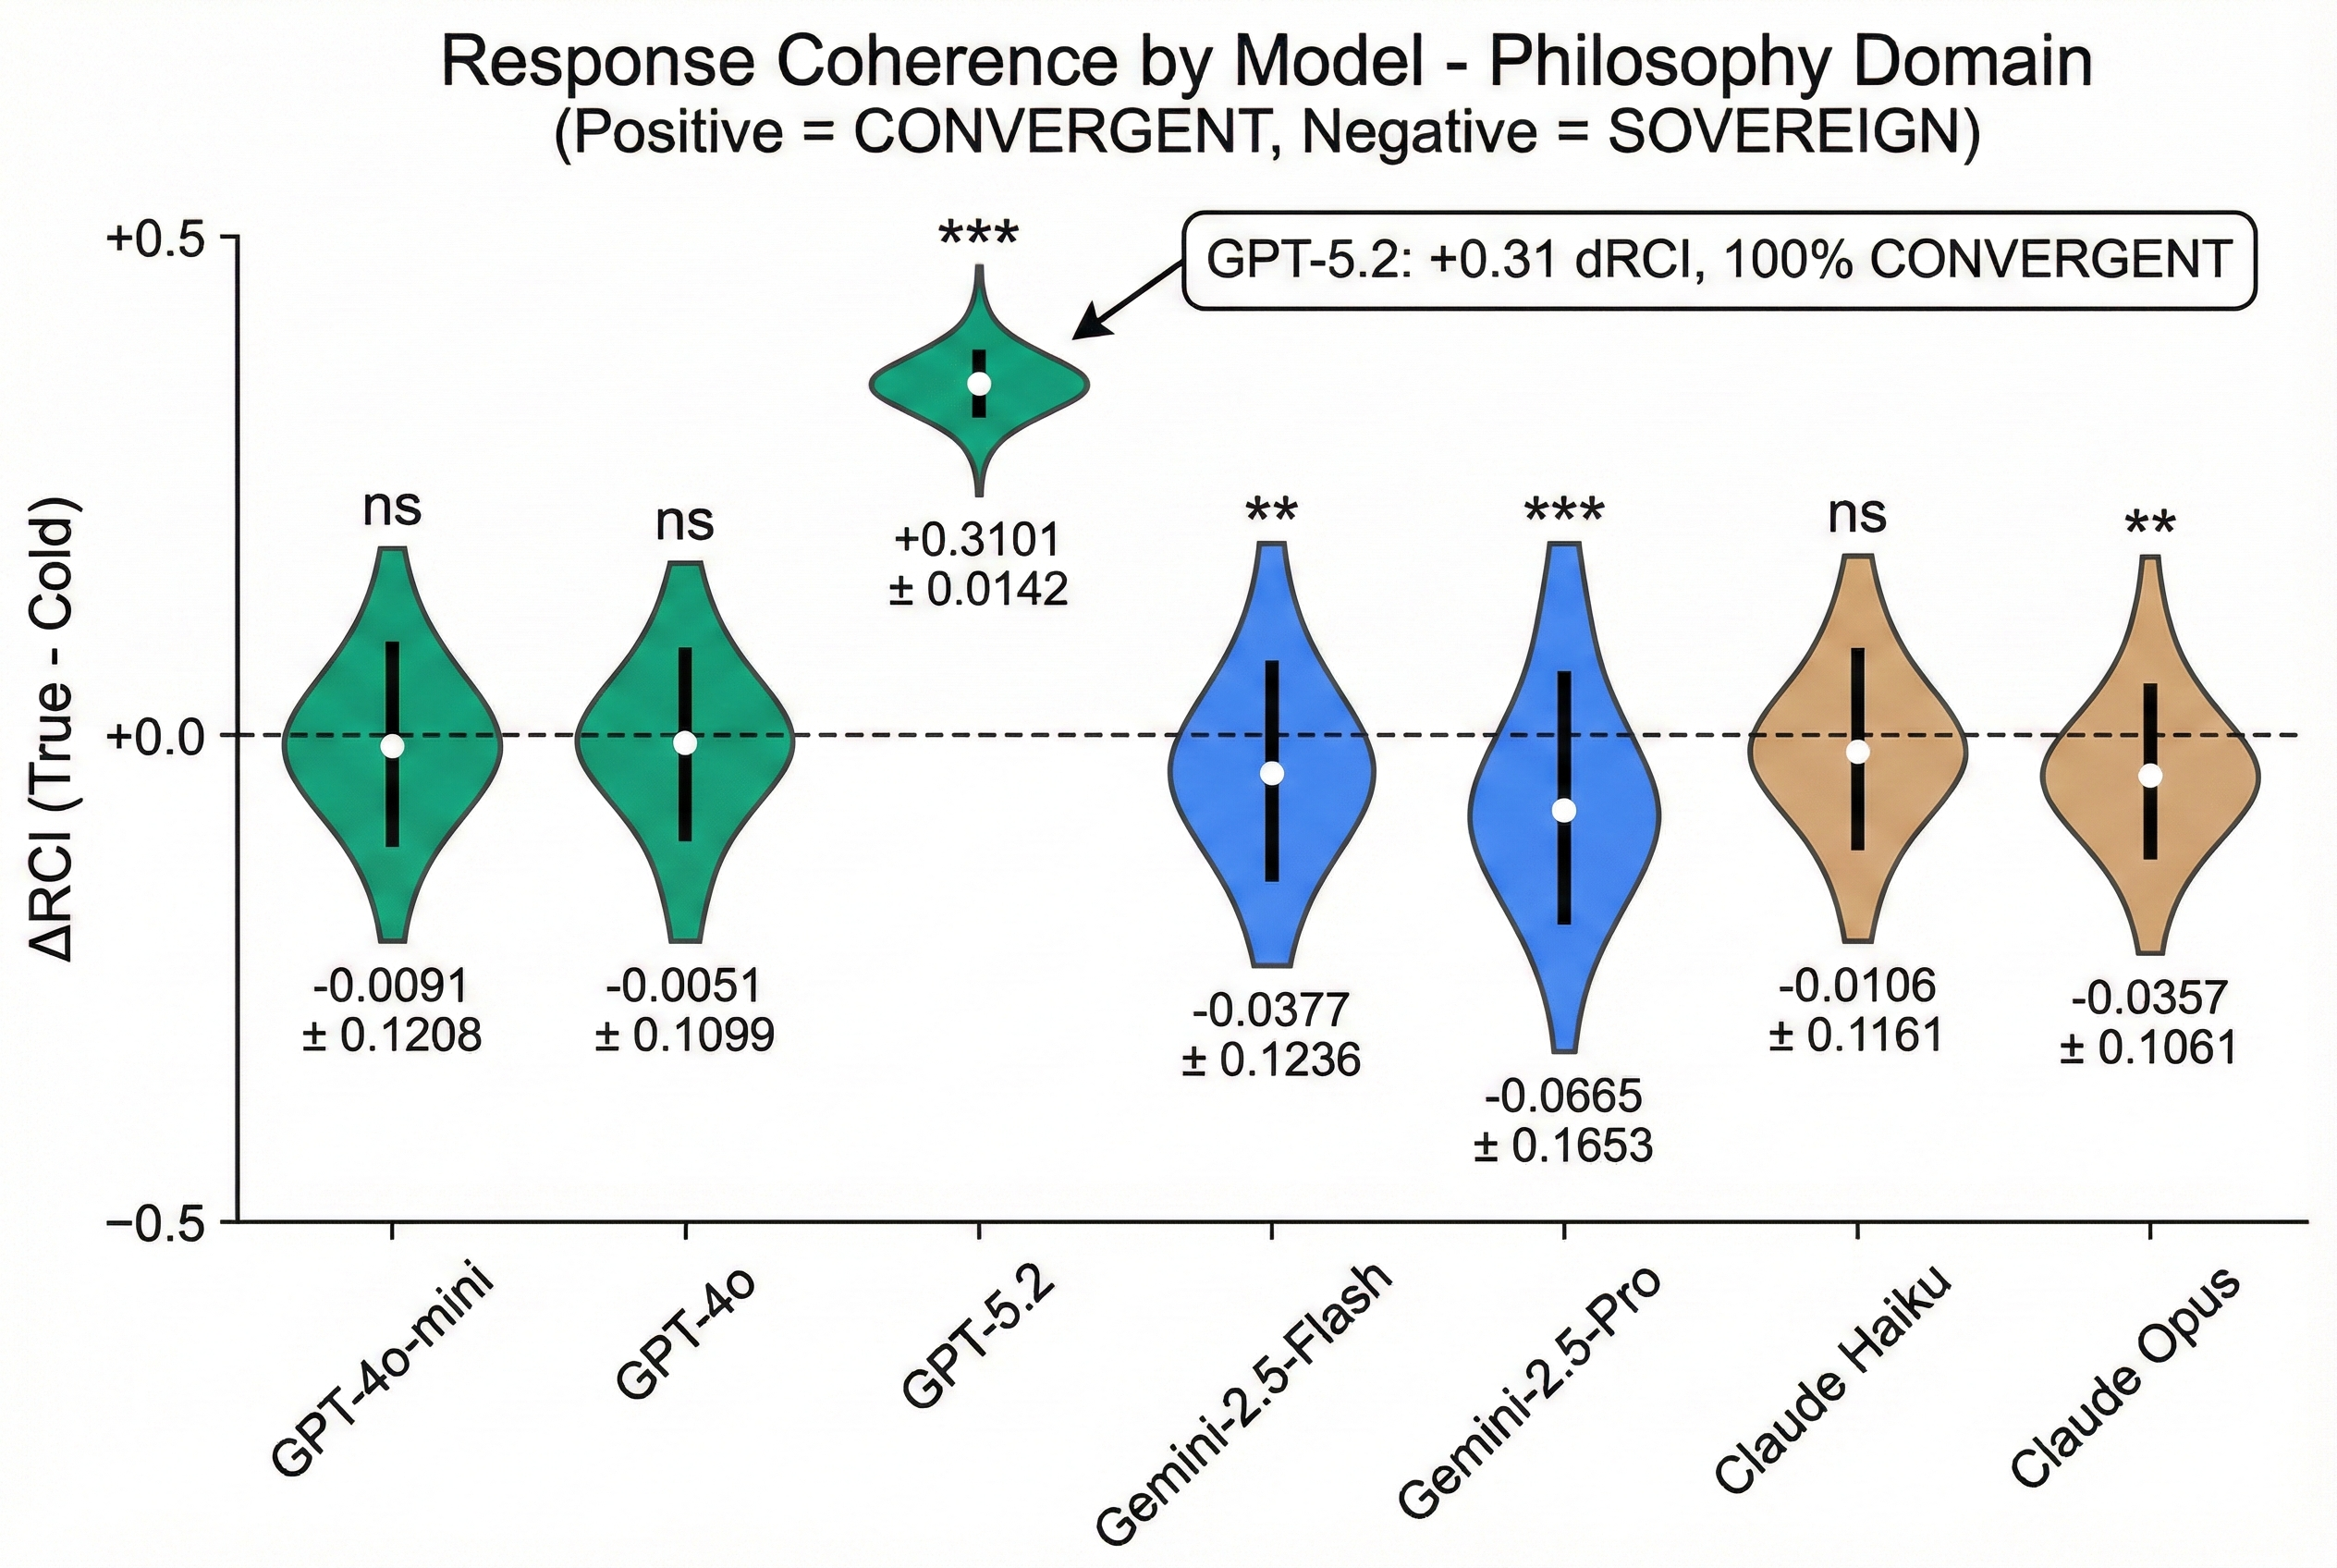
\includegraphics[width=0.95\textwidth]{fig1_philosophy_violin.png}
\caption{Response Coherence by Model ($\Delta$RCI Distribution) - Philosophy Domain. Distribution of $\Delta$RCI values across 100 trials for each model, color-coded by vendor (OpenAI: green, Google: blue, Anthropic: tan). GPT-5.2 shows uniquely tight distribution at +0.31 with 100\% CONVERGENT trials. Significance markers: *** $p$ < 0.001, ** $p$ < 0.01, ns = not significant.}
\label{fig:philosophy_violin}
\end{figure}

\begin{figure}[H]
\centering
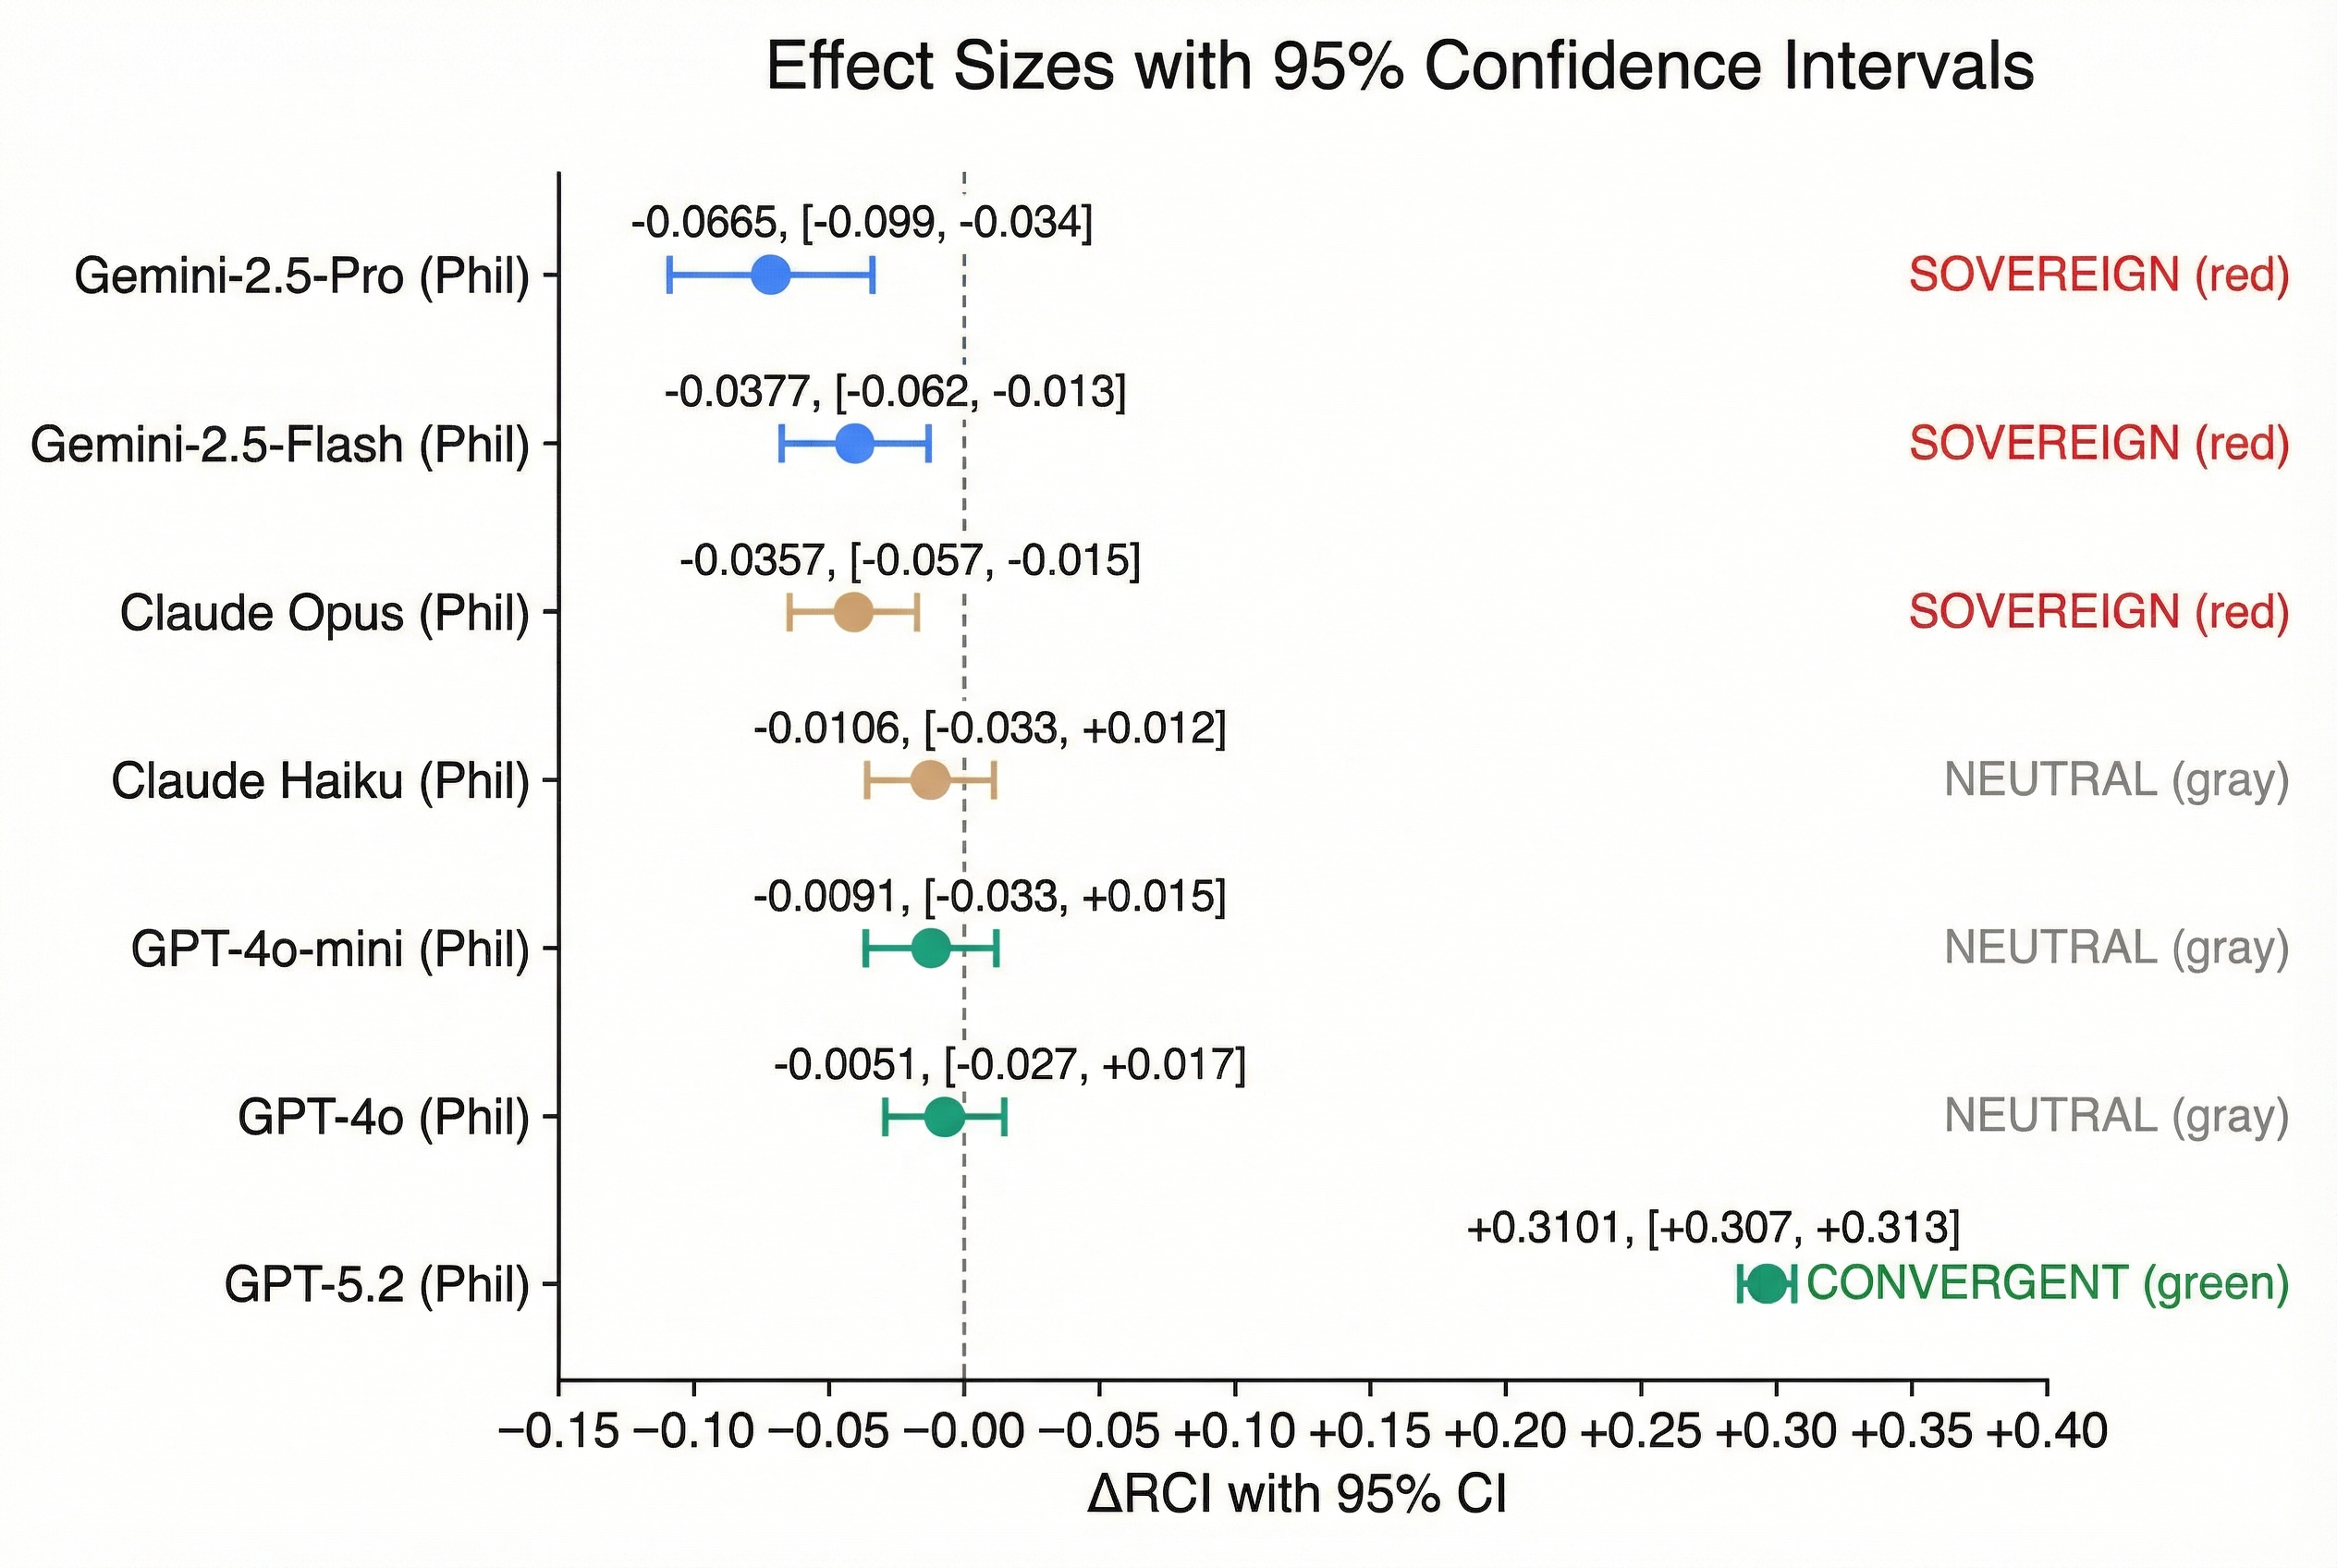
\includegraphics[width=0.95\textwidth]{fig2_effect_sizes_ci.png}
\caption{Effect Sizes with 95\% Confidence Intervals - Philosophy Domain. Mean $\Delta$RCI with 95\% confidence intervals for each model. GPT-5.2 stands alone as CONVERGENT with CI entirely above zero. Points crossing zero indicate NEUTRAL patterns; points entirely below zero indicate SOVEREIGN patterns.}
\label{fig:effect_sizes}
\end{figure}

\subsection{Medical Domain: CONVERGENT Patterns}

\begin{table}[H]
\centering
\caption{Medical Domain Results (50 trials per model). 95\% CI computed via bootstrap (10,000 resamples).}
\begin{tabular}{lccccc}
\toprule
\textbf{Model} & \textbf{Mean $\Delta$RCI} & \textbf{95\% CI} & \textbf{Pattern} & \textbf{Conv\%} & \textbf{$p$-value} \\
\midrule
GPT-4o & +0.299 & [0.296, 0.302] & CONVERGENT & 100\% & $<$10$^{-48}$ \\
GPT-4o-mini & +0.319 & [0.316, 0.322] & CONVERGENT & 100\% & $<$10$^{-52}$ \\
\textbf{GPT-5.2} & \textbf{+0.379} & \textbf{[0.373, 0.385]} & \textbf{CONVERGENT} & \textbf{100\%} & \textbf{$<$10$^{-46}$} \\
Claude Haiku & +0.340 & [0.337, 0.343] & CONVERGENT & 100\% & $<$10$^{-42}$ \\
Claude Opus & +0.339 & [0.334, 0.344] & CONVERGENT & 100\% & $<$10$^{-40}$ \\
Gemini 2.5 Flash & \textcolor{red}{-0.133} & \textcolor{red}{[-0.140, -0.126]} & \textcolor{red}{SOVEREIGN} & \textcolor{red}{0\%} & $<$10$^{-37}$ \\
\bottomrule
\end{tabular}
\label{tab:medical}
\end{table}

In medicine, most models show strong CONVERGENT patterns---context is essential for clinical reasoning. Gemini 2.5 Flash is the sole exception, maintaining SOVEREIGN behavior even in guideline-anchored content. Gemini 2.5 Pro was blocked by safety filters for medical prompts.

\begin{figure}[H]
\centering
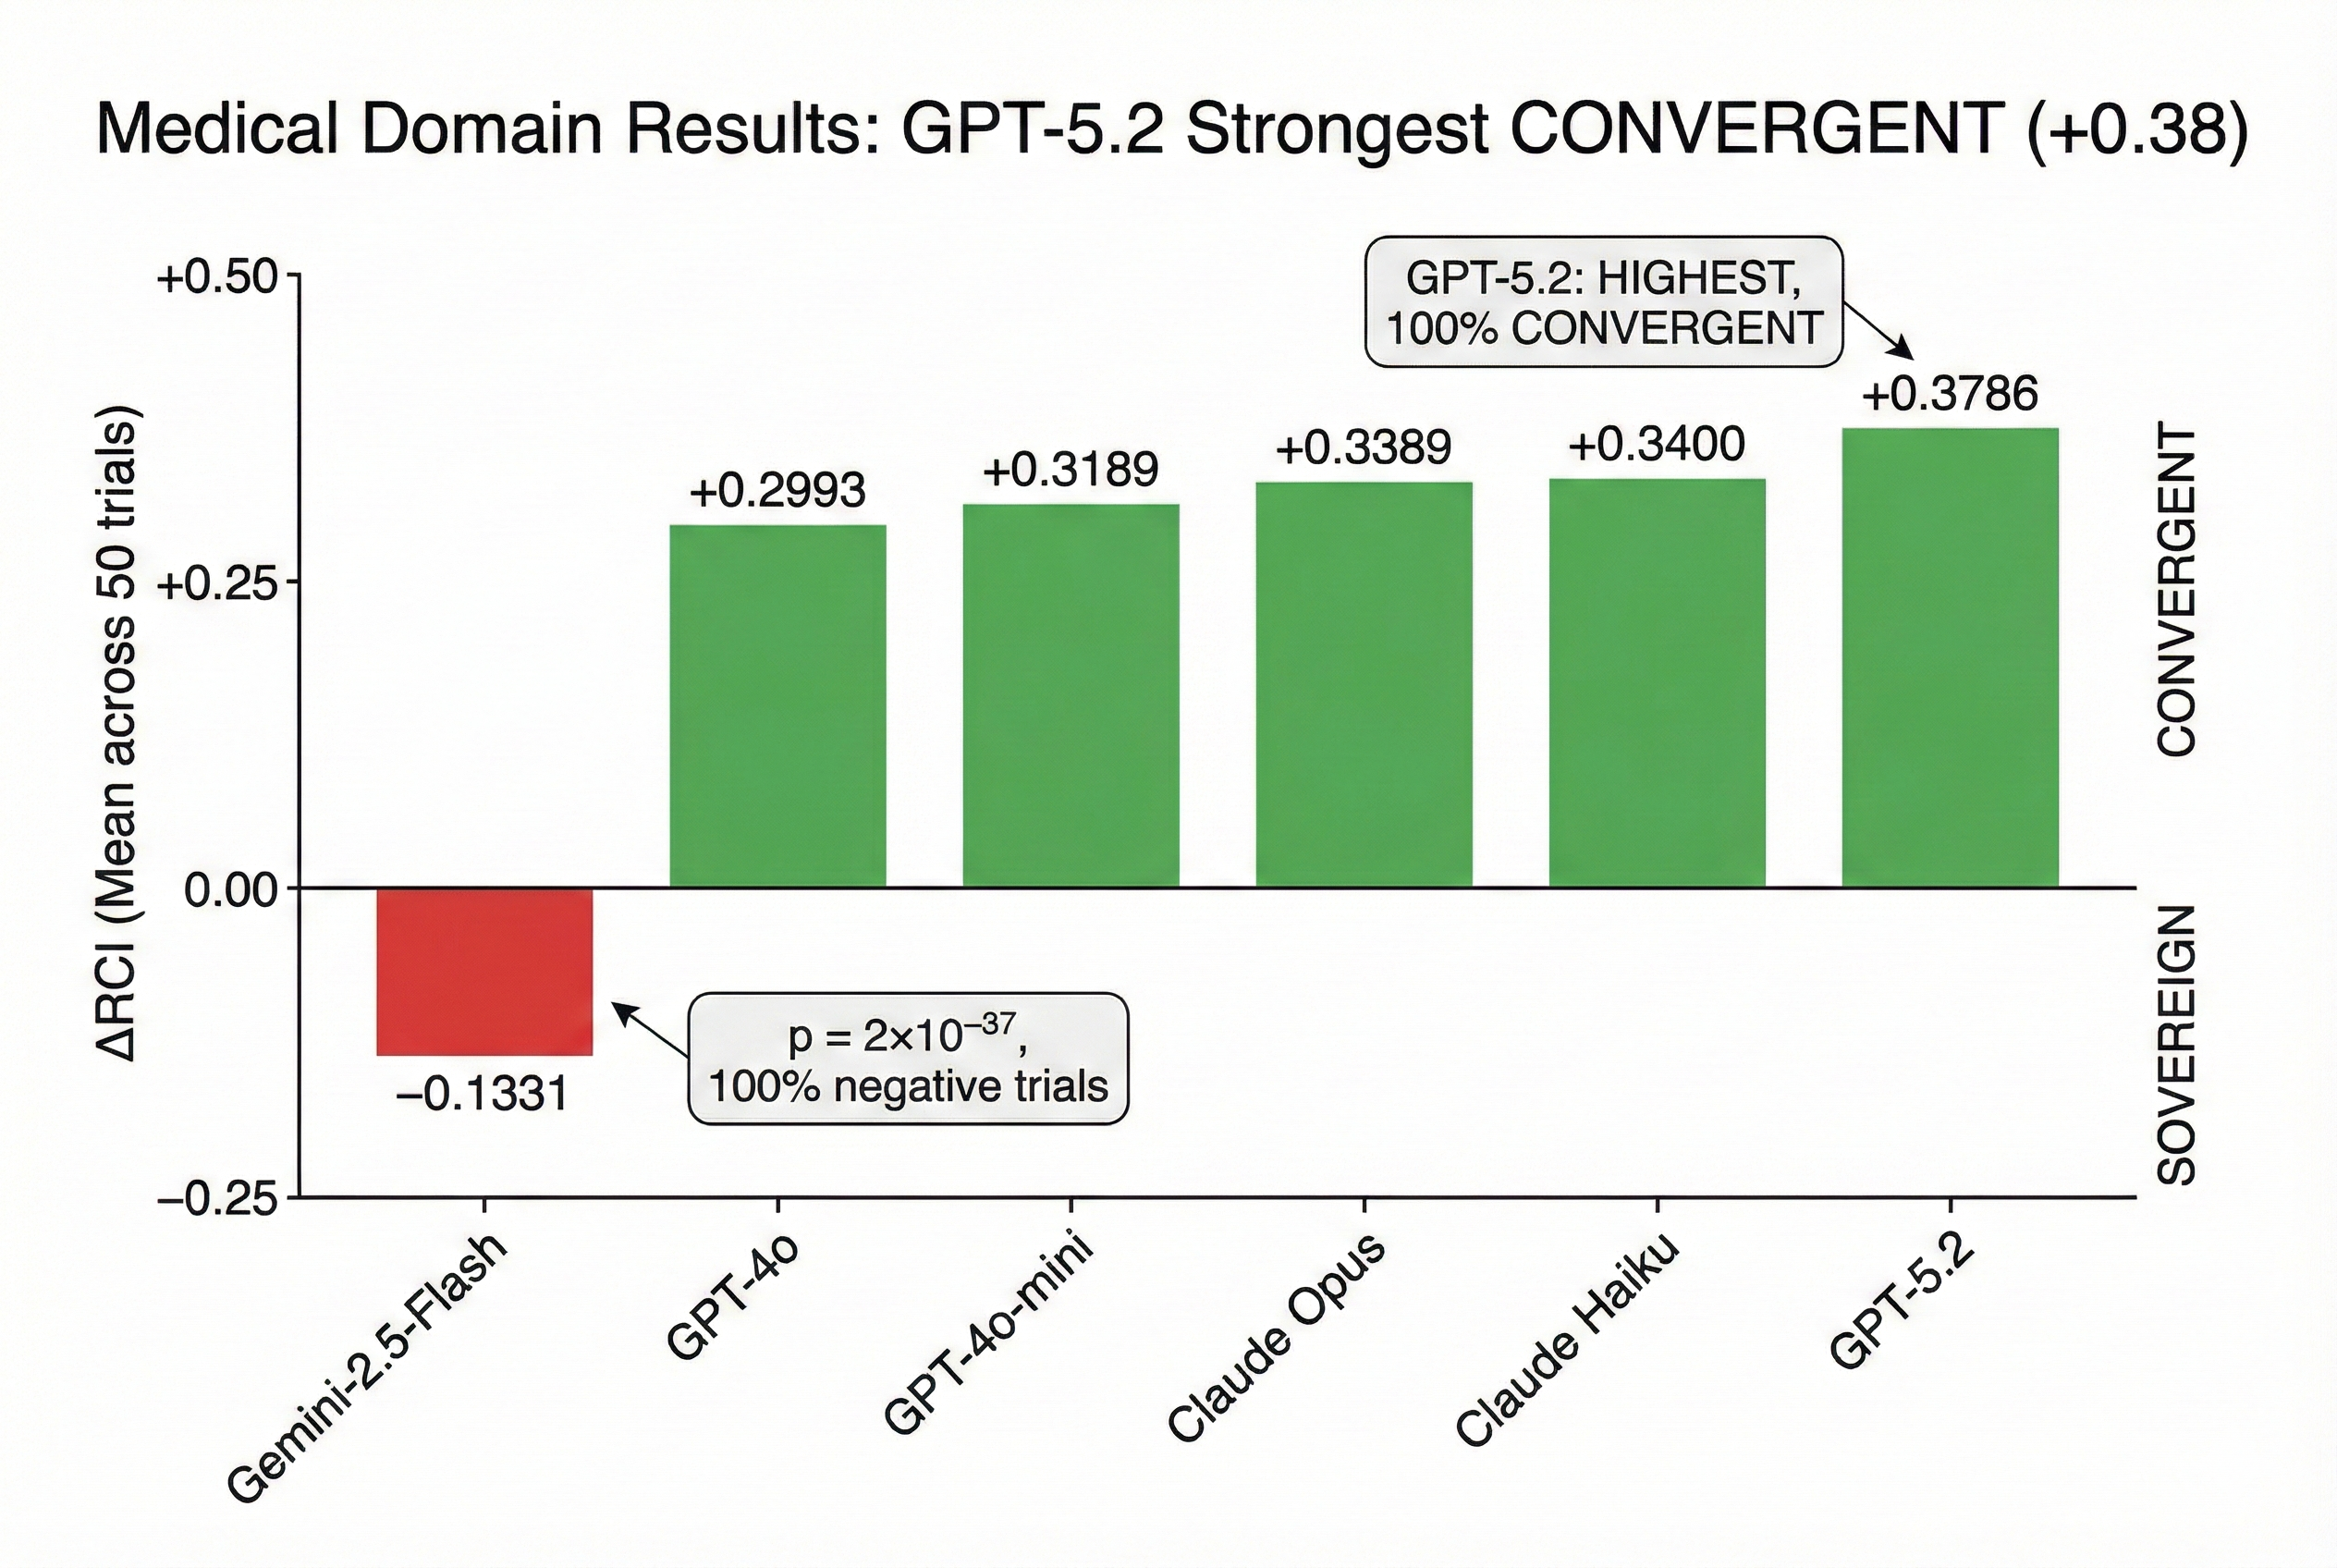
\includegraphics[width=0.95\textwidth]{fig7_medical_results.png}
\caption{Medical Domain Results: GPT-5.2 Strongest CONVERGENT. All models except Gemini 2.5 Flash show strong CONVERGENT patterns (+0.30 to +0.38). Gemini Flash uniquely SOVEREIGN (-0.133, $p$=2$\times$10$^{-37}$, 100\% negative trials) even in guideline-anchored medical domain.}
\label{fig:medical_results}
\end{figure}

\subsection{Cross-Domain Comparison: The Flip}

\begin{table}[H]
\centering
\caption{Cross-Domain $\Delta$RCI Shift (Same Model, Different Domains). Cohen's $d$ interpretation: 0.2=small, 0.5=medium, 0.8=large (Cohen, 1988).}
\begin{tabular}{lcccc}
\toprule
\textbf{Model} & \textbf{Philosophy} & \textbf{Medical} & \textbf{Shift} & \textbf{Cohen's $d$} \\
\midrule
GPT-4o & -0.005 (NEUTRAL) & +0.299 (CONV) & +0.304 & 2.78 (very large) \\
GPT-4o-mini & -0.009 (NEUTRAL) & +0.319 (CONV) & +0.328 & 2.71 (very large) \\
\textbf{GPT-5.2} & \textbf{+0.310 (CONV)} & \textbf{+0.379 (CONV)} & \textbf{+0.069} & \textbf{3.82 (very large)} \\
Claude Haiku & -0.011 (NEUTRAL) & +0.340 (CONV) & +0.351 & 4.25 (very large) \\
Claude Opus & -0.036 (SOV) & +0.339 (CONV) & +0.375 & 4.02 (very large) \\
Gemini Flash & -0.038 (SOV) & -0.133 (SOV) & -0.095 & 0.42 (small) \\
\bottomrule
\end{tabular}
\label{tab:crossdomain}
\end{table}

Five of six models ``flip'' behavioral mode between domains, with Cohen's $d$ > 2.7. This massive effect size (d > 0.8 is typically ``large''; Cohen, 1988) demonstrates that domain fundamentally alters context utilization. Gemini Flash alone maintains SOVEREIGN behavior in both domains.

\begin{figure}[H]
\centering
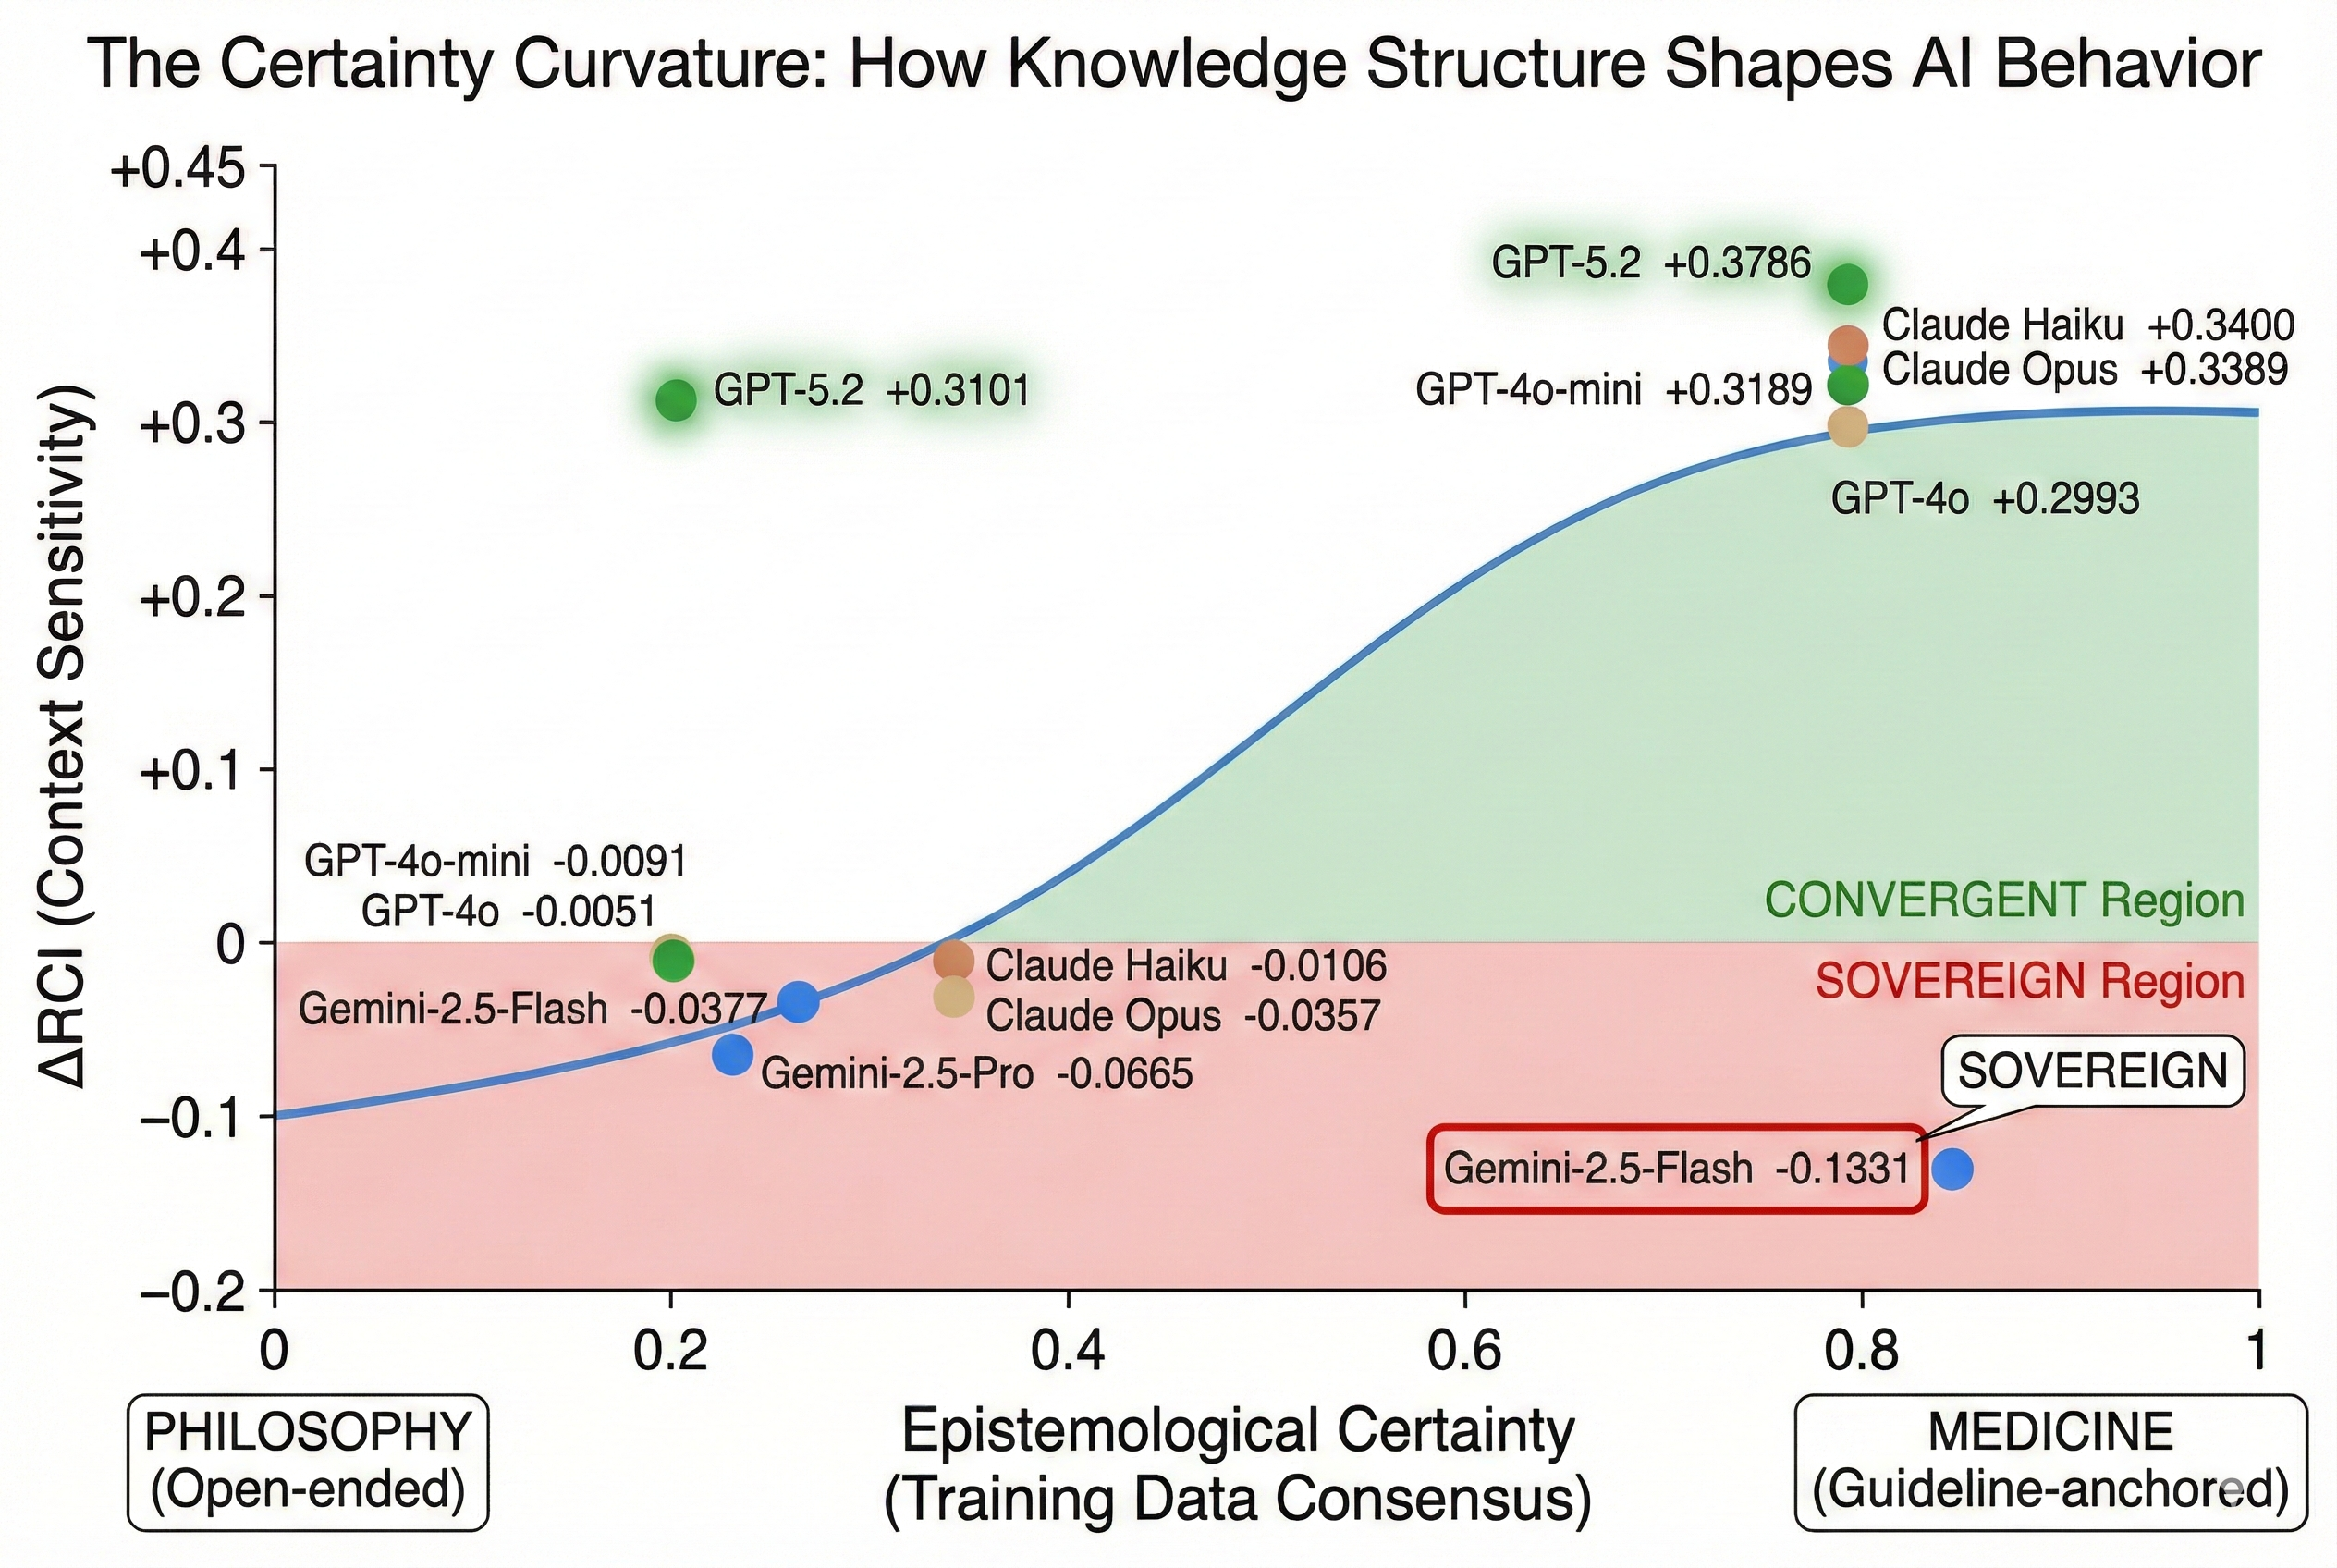
\includegraphics[width=0.95\textwidth]{fig4_certainty_curvature.png}
\caption{The Certainty Curvature: How Knowledge Structure Shapes AI Behavior. S-curve shows theoretical prediction of $\Delta$RCI as function of epistemological certainty. Philosophy (low certainty) clusters near zero/negative; Medicine (high certainty) shows strong positive $\Delta$RCI. GPT-5.2 uniquely CONVERGENT in both domains. Gemini Flash remains SOVEREIGN even in medical domain (red square).}
\label{fig:certainty_curvature}
\end{figure}

\subsection{GPT-5.2: The Outlier}

GPT-5.2 exhibits unique characteristics:

\begin{itemize}
    \item \textbf{100\% CONVERGENT} in both philosophy AND medicine (only model)
    \item \textbf{150 trials}, zero SOVEREIGN or NEUTRAL trials
    \item \textbf{Lowest variance:} $\sigma$ = 0.014 (philosophy), $\sigma$ = 0.021 (medical); CV = 0.046, 0.055 respectively
    \item \textbf{Comparison:} Other models show CV = 2.5--21.5
\end{itemize}

This suggests architectural or training differences in the GPT-5 generation that ``lock'' convergent behavior regardless of domain.

\begin{figure}[H]
\centering
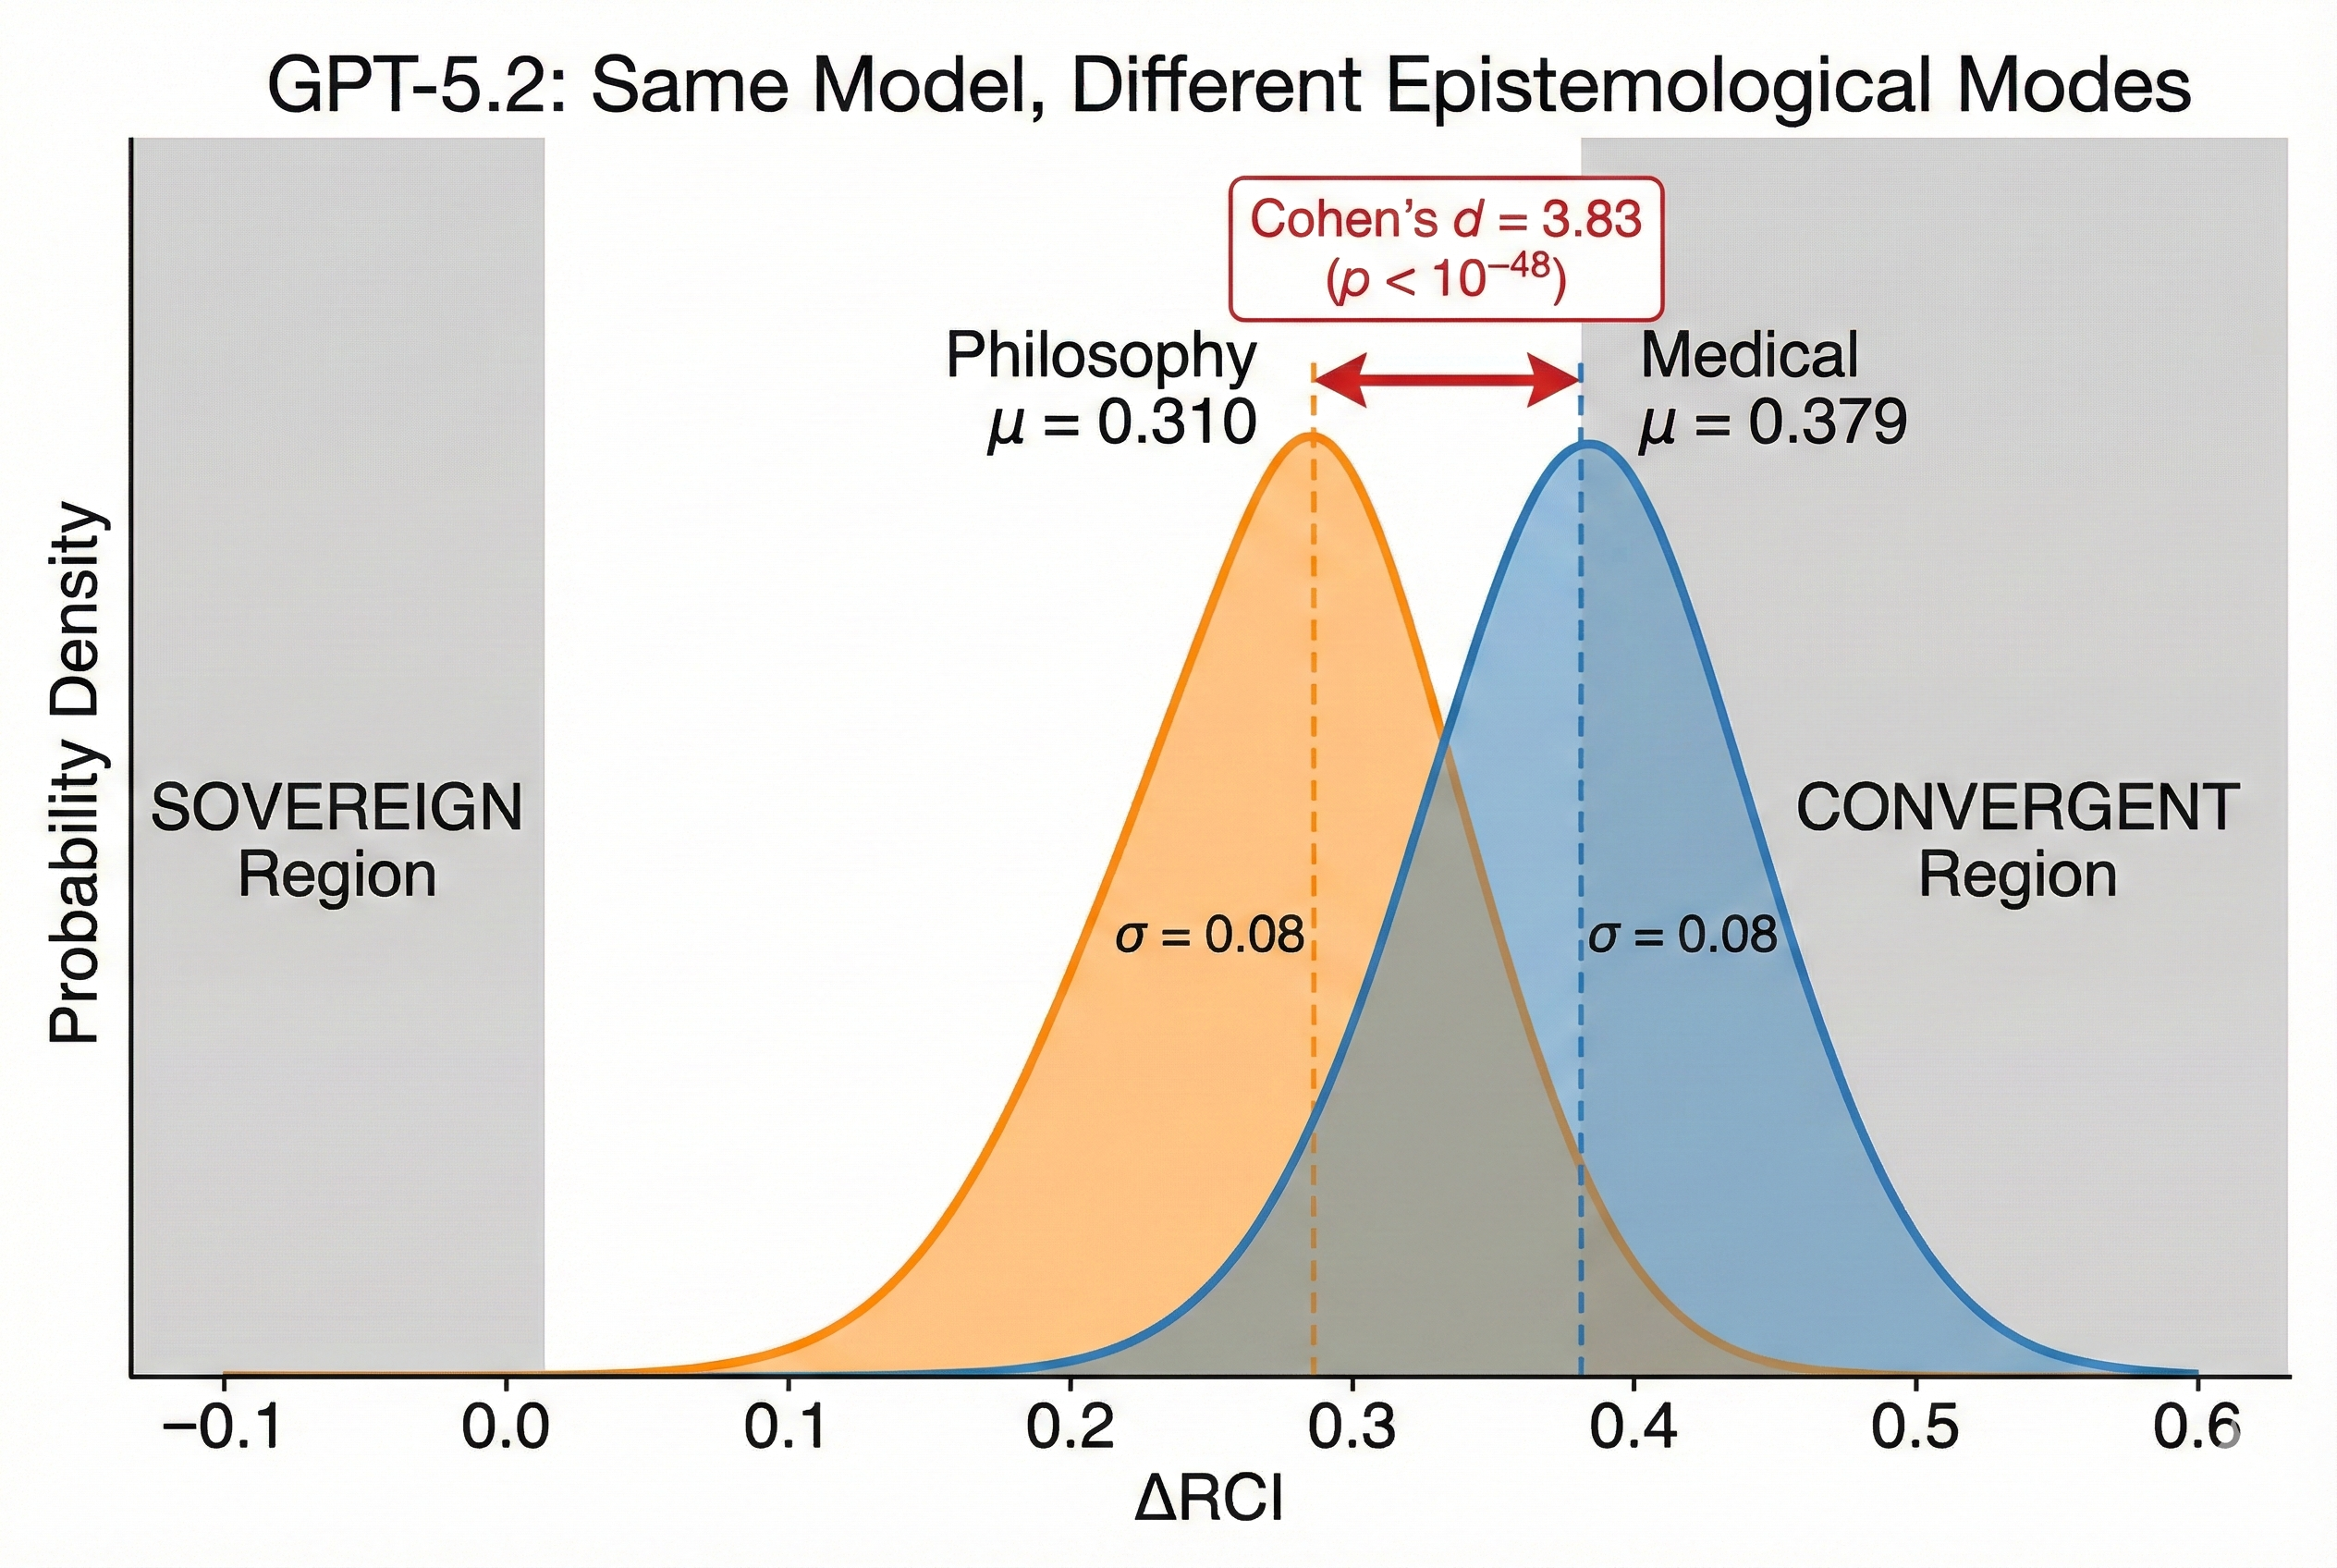
\includegraphics[width=0.95\textwidth]{fig6_gpt52_domains.png}
\caption{GPT-5.2: Same Model, Different Epistemological Modes. Both Philosophy ($\mu$=0.310) and Medical ($\mu$=0.379) domains show CONVERGENT behavior with Cohen's $d$=3.82. Unlike other models that flip between domains, GPT-5.2 maintains consistent convergence regardless of epistemological context.}
\label{fig:gpt52_domains}
\end{figure}

\subsection{SCRAMBLED Condition: Coherence Matters}

\begin{table}[H]
\centering
\caption{TRUE vs SCRAMBLED vs COLD Comparison. Values normalized to TRUE condition within each model (TRUE=1.000) for interpretability; raw RCI values available in repository.}
\begin{tabular}{lcccc}
\toprule
\textbf{Model} & \textbf{TRUE} & \textbf{SCRAMBLED} & \textbf{COLD} & \textbf{Pattern} \\
\midrule
GPT-5.2 (Phil) & 1.000 & 0.759 & 0.690 & TRUE > SCRAM > COLD \\
GPT-5.2 (Med) & 1.000 & 0.768 & 0.621 & TRUE > SCRAM > COLD \\
GPT-4o (Med) & 1.000 & 0.829 & 0.701 & TRUE > SCRAM > COLD \\
Claude Haiku (Med) & 1.000 & 0.729 & 0.660 & TRUE > SCRAM > COLD \\
\textcolor{red}{Gemini Flash (Med)} & \textcolor{red}{0.555} & \textcolor{red}{0.560} & \textcolor{red}{0.688} & \textcolor{red}{COLD > SCRAM $\approx$ TRUE} \\
\bottomrule
\end{tabular}
\label{tab:scrambled}
\end{table}

For CONVERGENT models: TRUE > SCRAMBLED > COLD ($p$ < 10$^{-30}$). This demonstrates that coherent history outperforms scrambled history---it is not mere token presence but meaningful structure that enhances responses.

For SOVEREIGN models (Gemini Flash): COLD > SCRAMBLED $\approx$ TRUE. Fresh start outperforms any history, coherent or not. This exception highlights that the coherence benefit is pattern-dependent.

\subsection{Vendor Effects}

One-way ANOVA across vendors (philosophy domain, $n$=700): $F$(2,697) = 6.52, $p$ = 0.0015. Significant vendor-level differences in context utilization strategy exist even controlling for model tier.

\begin{figure}[H]
\centering
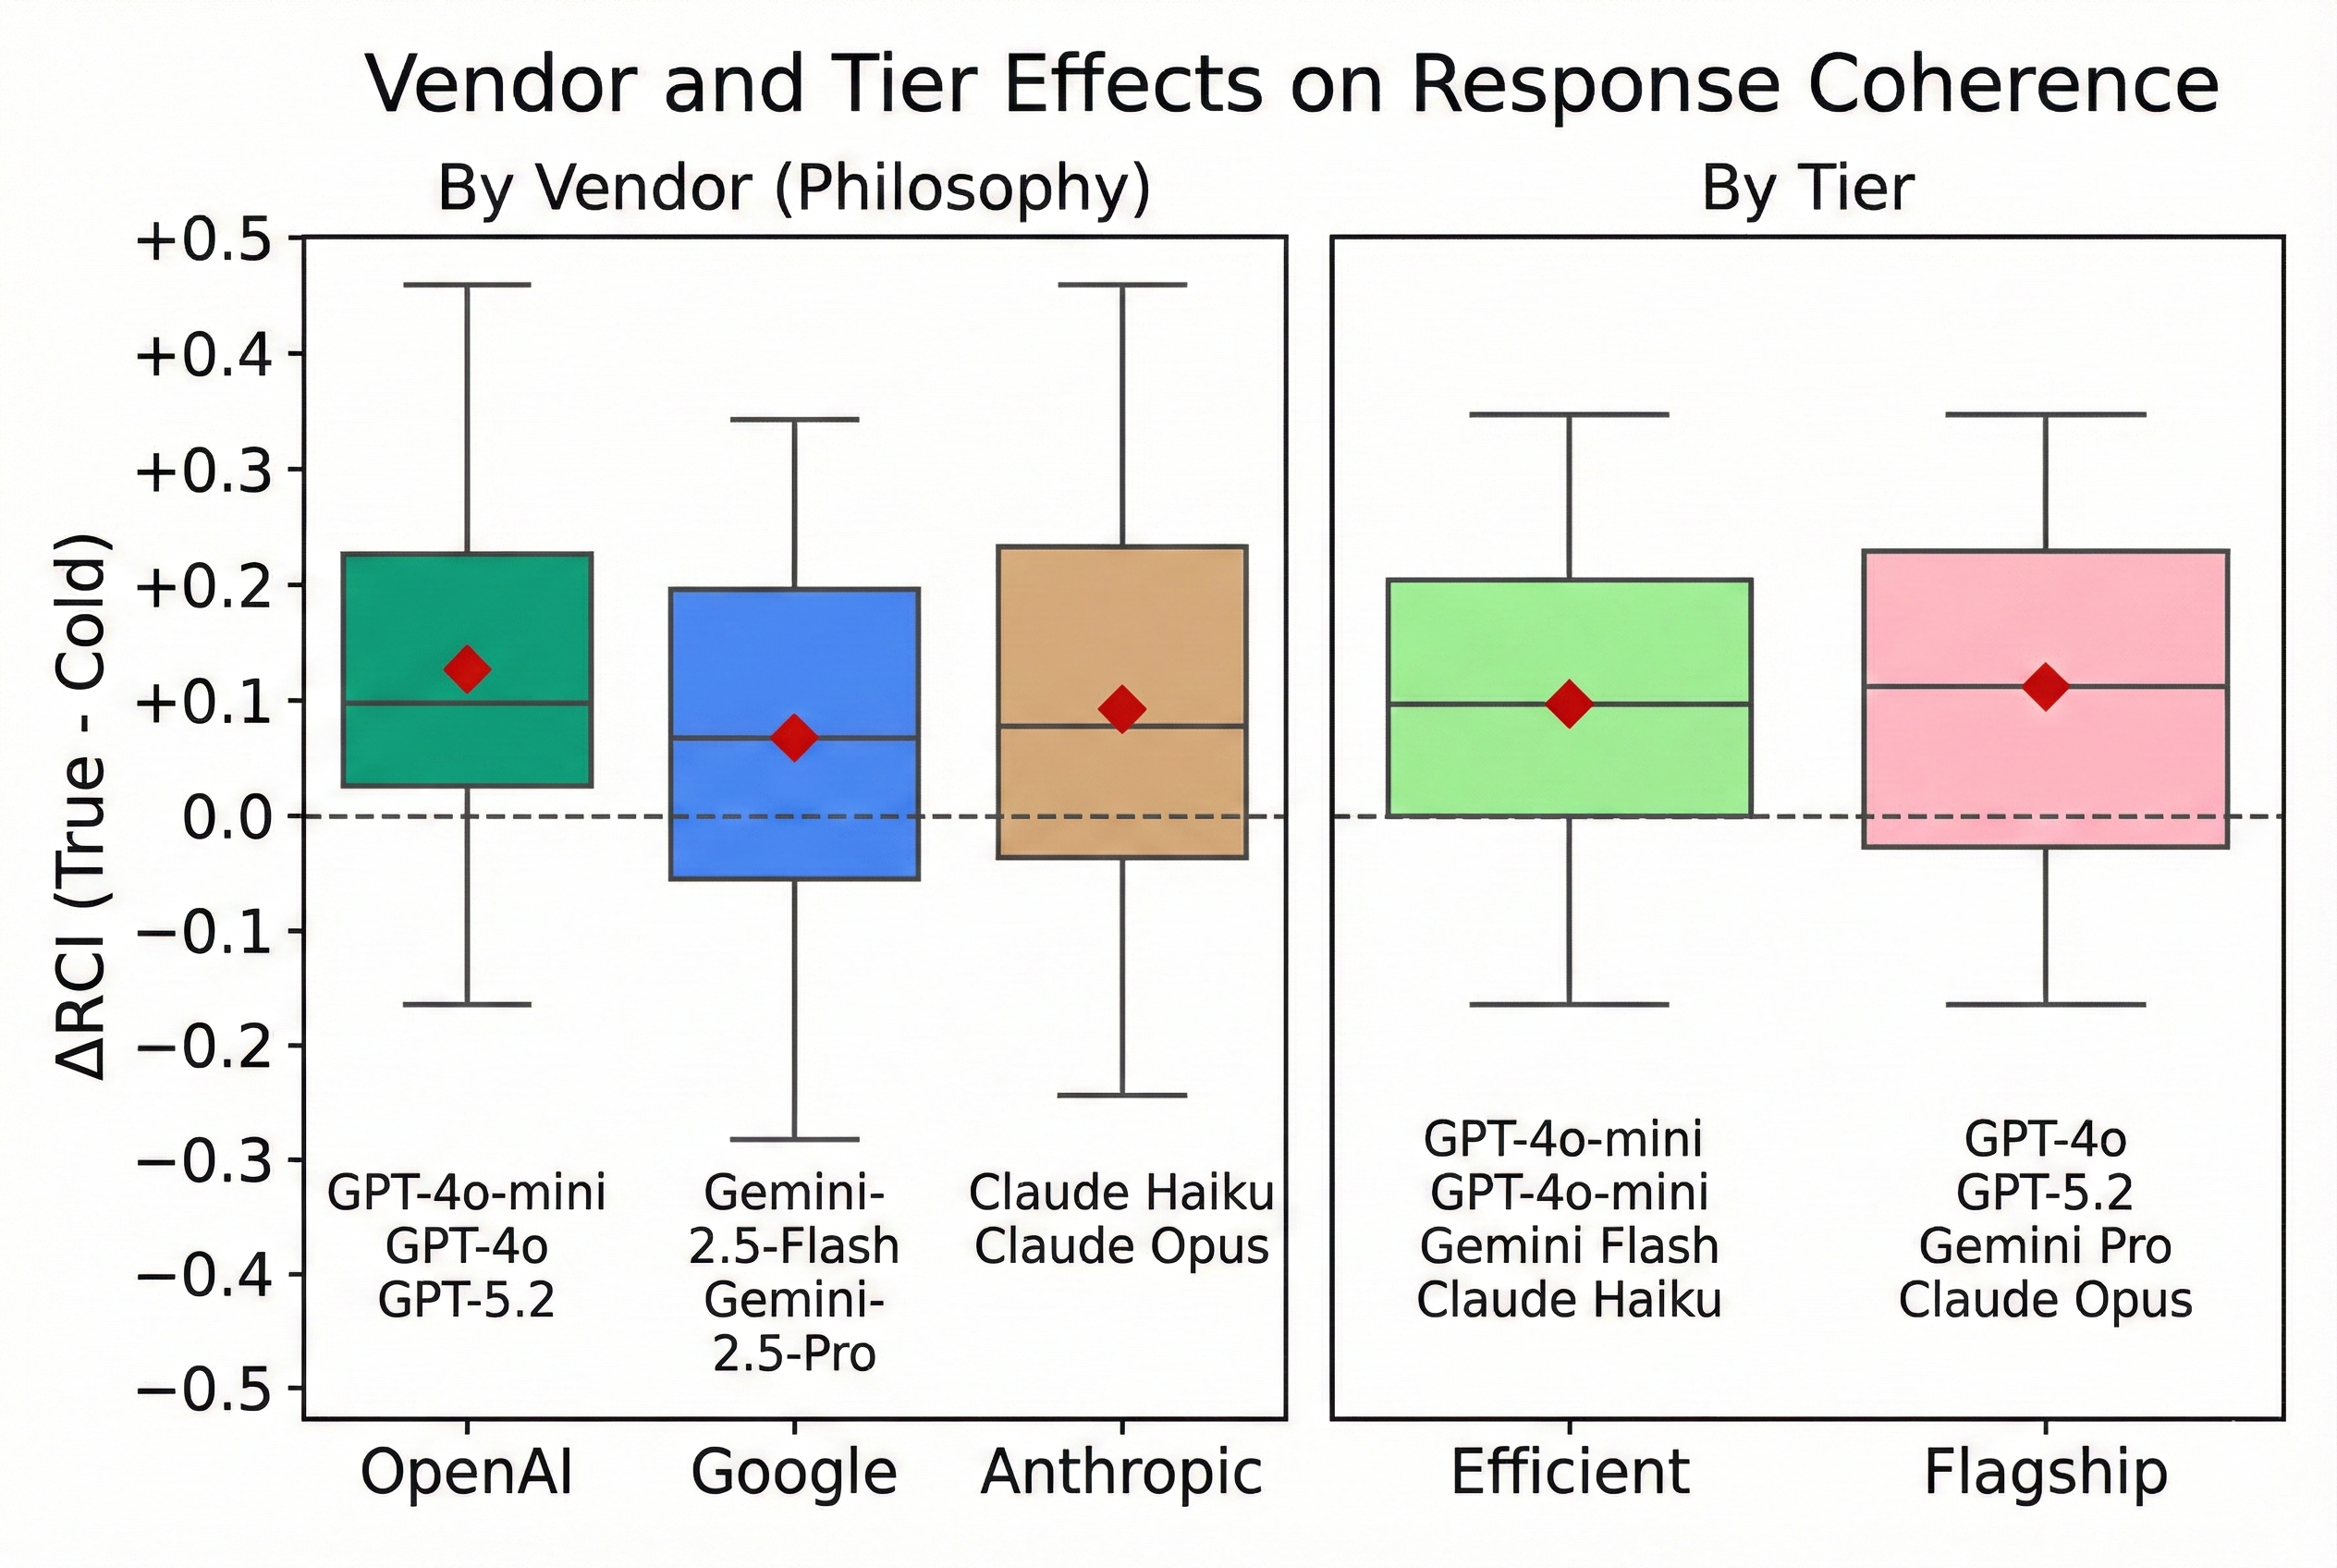
\includegraphics[width=0.95\textwidth]{fig3_vendor_tier.png}
\caption{Vendor and Tier Effects on Response Coherence. Left panel: $\Delta$RCI distribution by vendor, with OpenAI pulled upward by GPT-5.2. Right panel: $\Delta$RCI distribution by model tier (Efficient vs Flagship).}
\label{fig:vendor_tier}
\end{figure}

\subsection{Gemini Safety Filter Progression}

\begin{table}[H]
\centering
\caption{Gemini Safety Filter Observations}
\begin{tabular}{lcc}
\toprule
\textbf{Model} & \textbf{Philosophy} & \textbf{Medical} \\
\midrule
Gemini 2.5 Flash & $\checkmark$ Allowed & $\checkmark$ Allowed \\
Gemini 2.5 Pro & $\checkmark$ Allowed & $\times$ Blocked \\
Gemini 3 Pro & $\times$ Blocked & $\times$ Blocked \\
\bottomrule
\end{tabular}
\label{tab:gemini_safety}
\end{table}

Progressive safety filtering: newer/larger Gemini models have more aggressive content restrictions.

\subsection{Statistical Robustness}

\textbf{Bonferroni correction:} With 42 tests (7 models $\times$ 3 condition pairs $\times$ 2 domains), adjusted $\alpha$ = 0.05/42 = 0.00119. Main findings (GPT-5.2 both domains, all medical CONVERGENT except Gemini) survive correction.

\textbf{Power analysis:} For $n$=50, MDES = 0.0692; for $n$=100, MDES = 0.0489. All reported effects exceed these thresholds.

% ============================================================================
\section{Discussion}
% ============================================================================

\subsection{Epistemological Relativity}

We propose \textbf{Epistemological Relativity} as a theoretical framework: AI behavior is not absolute but relative to the epistemological structure of the task.

\textbf{Proposed mechanism:} LLMs learn not just answers but \textit{certainty structure} from training data (Ouyang et al., 2022). High-consistency domains (medicine: one correct protocol) induce CONVERGENT behavior---the model trusts accumulated context. Low-consistency domains (philosophy: many valid views) induce SOVEREIGN behavior---the model discounts potentially contradictory history.

This hypothesis requires further testing through controlled training experiments, but it parsimoniously explains our observations.

\subsubsection{A Note on Response Quality}

The SOVEREIGN pattern should not be interpreted as producing inferior responses. Preliminary analysis of insight quality scores (available for philosophy trials) reveals that Claude Opus---classified as SOVEREIGN---maintained the highest consistent response quality across all 30 prompts, never dropping below 1.0 after prompt 2. Meanwhile, all models showed similar entanglement growth ($\sim$400\%), indicating they increasingly referenced conversational context regardless of $\Delta$RCI pattern:

\begin{table}[H]
\centering
\small
\begin{tabular}{lccc}
\toprule
\textbf{Model} & \textbf{Pattern} & \textbf{Insight Quality} & \textbf{Entanglement Growth} \\
\midrule
Claude Opus & SOVEREIGN & Highest, consistent & +432\% \\
GPT-4o & NEUTRAL & Variable, drops to 0 & +383\% \\
Gemini Pro & SOVEREIGN & Strong growth & +407\% \\
\bottomrule
\end{tabular}
\end{table}

This suggests SOVEREIGN models \textit{process} context but maintain independent reasoning trajectories---they listen without being swayed. Full analysis of response quality and entanglement dynamics will be presented in forthcoming work.

\subsection{The Two-Layer Model}

We propose AI context behavior operates through two layers:

\begin{enumerate}
    \item \textbf{Architecture Layer:} Base capacity for context processing (attention mechanisms, context window; Vaswani et al., 2017)
    \item \textbf{Epistemology Layer:} Learned certainty structure modulating how context is utilized
\end{enumerate}

GPT-5.2's unique pattern suggests architectural changes that bypass epistemological modulation, maintaining CONVERGENT behavior regardless of domain.

Gemini Flash's persistent SOVEREIGN pattern suggests architectural constraints (``small aperture'') that limit context utilization even when domain would otherwise encourage it.

\begin{figure}[H]
\centering
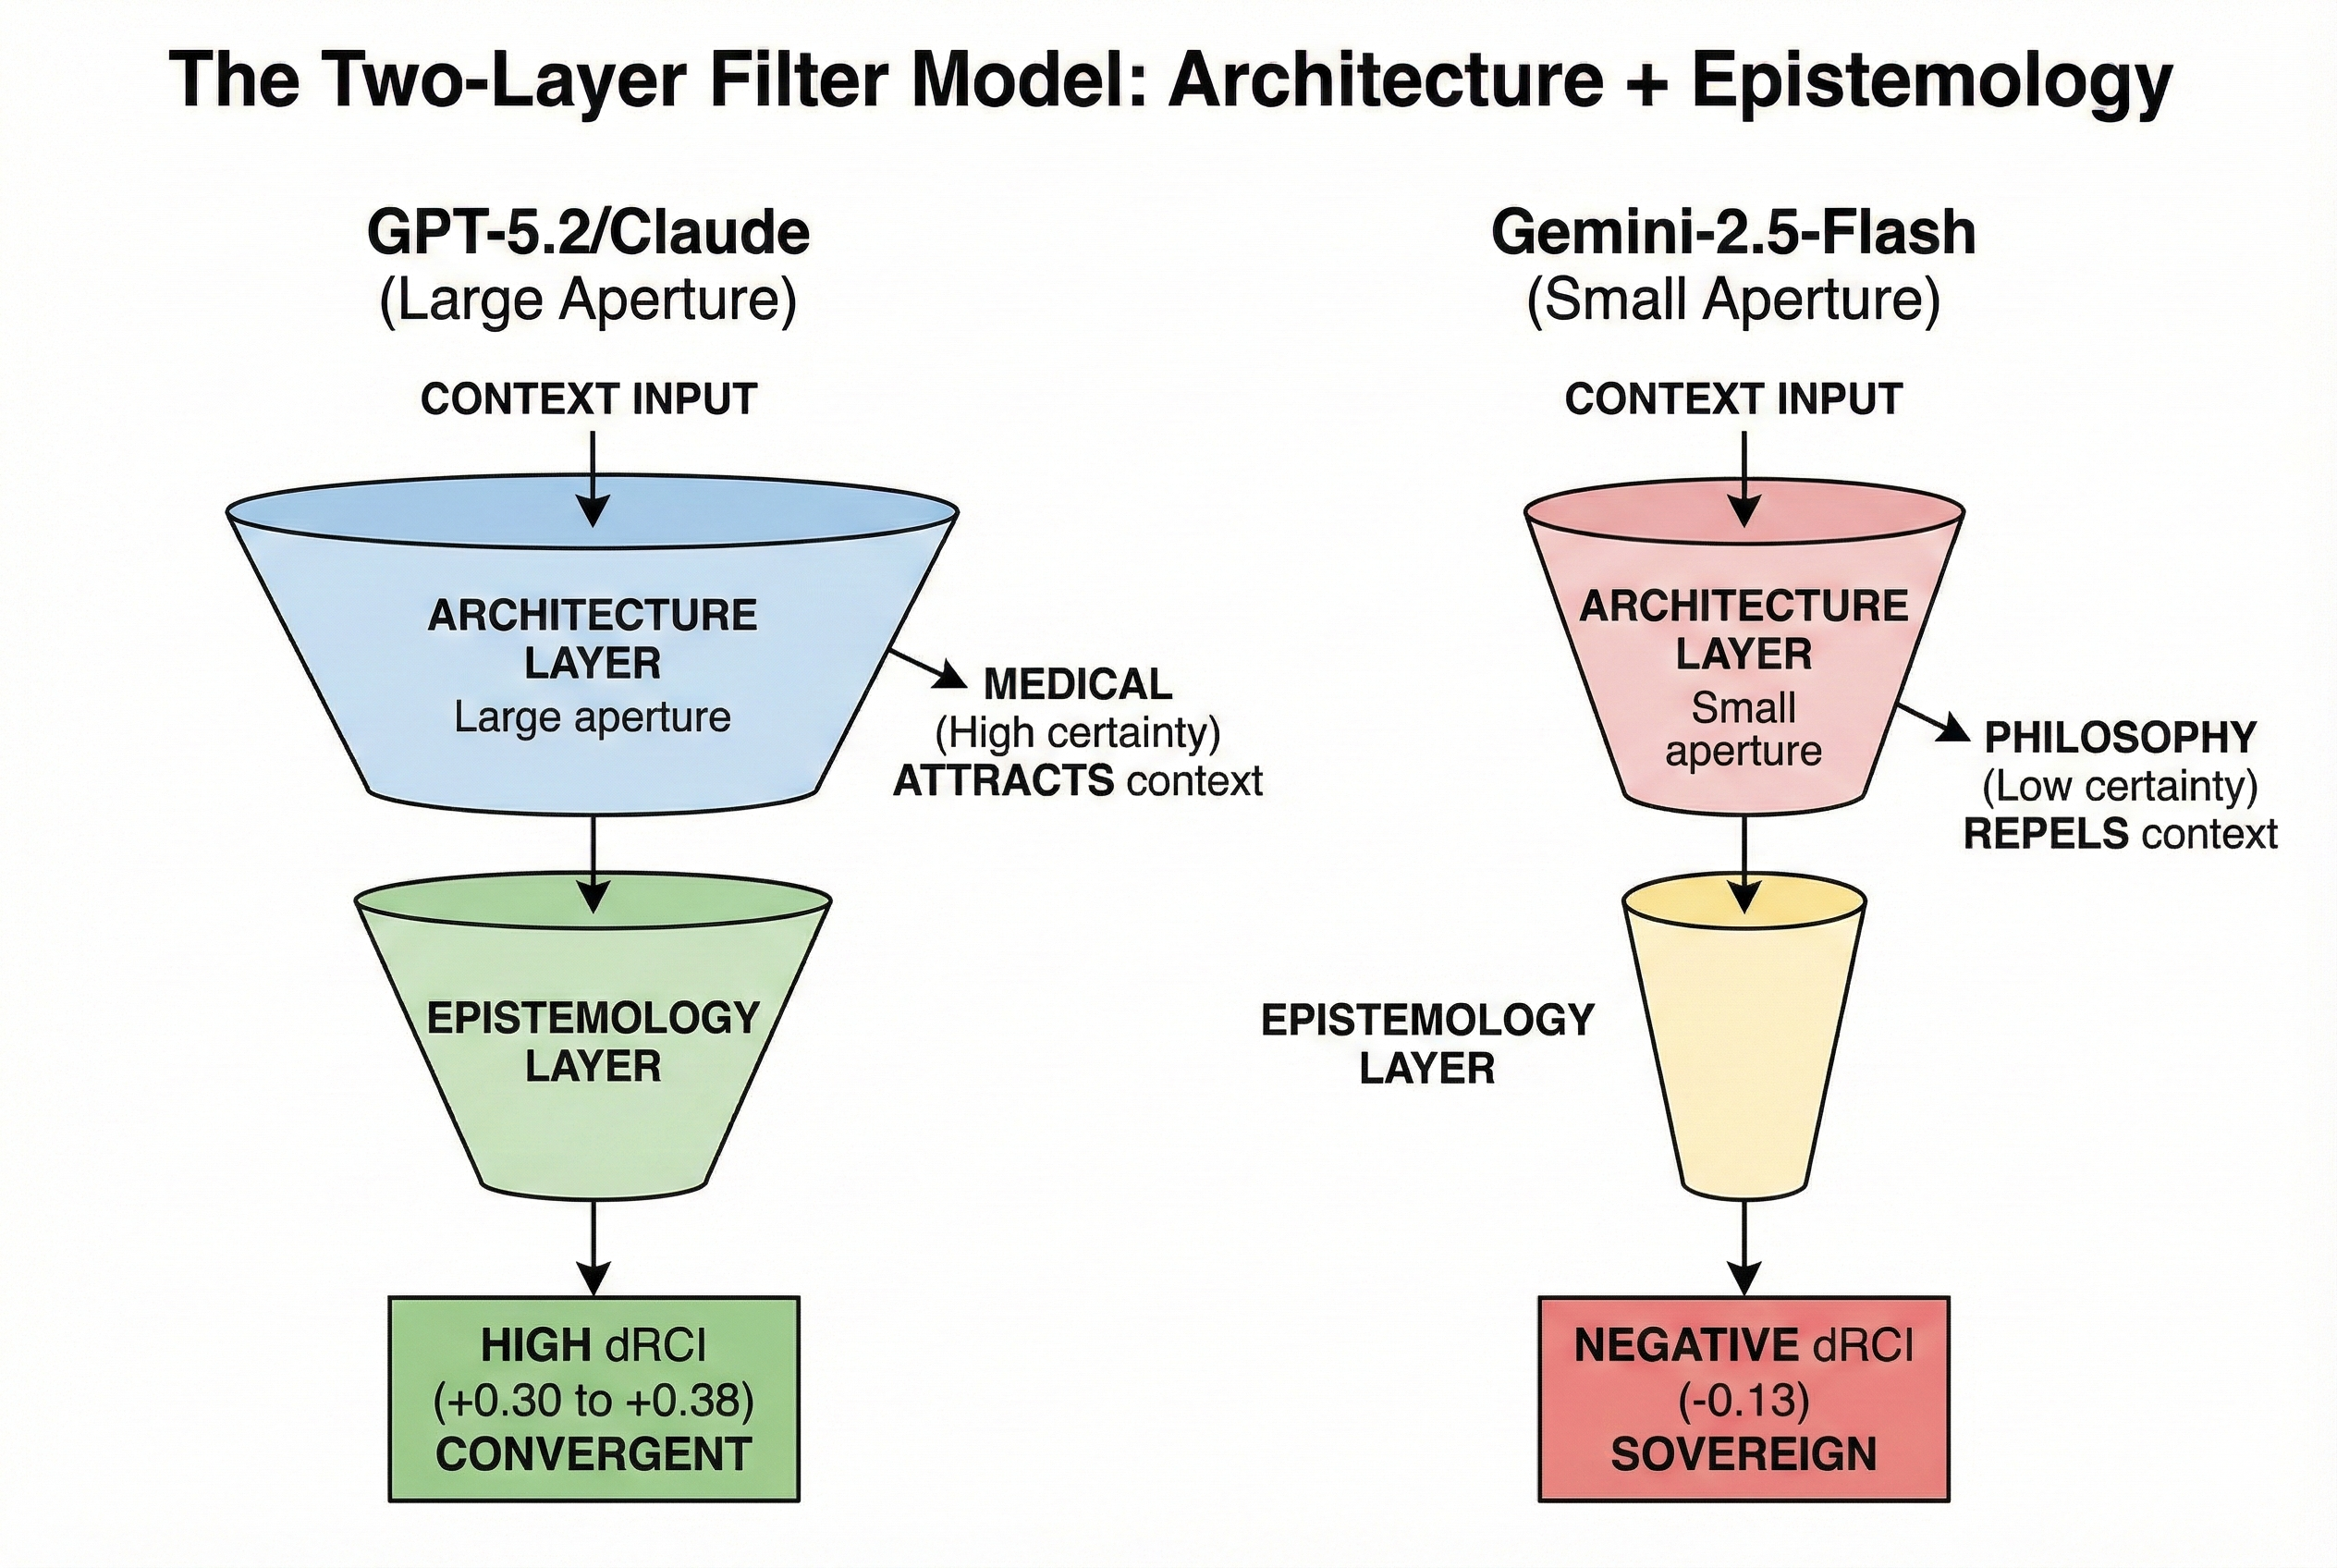
\includegraphics[width=0.95\textwidth]{fig5_two_layer_model.png}
\caption{The Two-Layer Filter Model: Architecture + Epistemology. Context utilization determined by two layers: (1) Architecture Layer (model design, attention mechanisms) and (2) Epistemology Layer (domain certainty structure). GPT-5.2/Claude have large aperture; Gemini Flash has small aperture limiting context use.}
\label{fig:two_layer_model}
\end{figure}

\subsection{Practical Applications}

\subsubsection{Prompt Engineering Guidelines}

\begin{itemize}
    \item \textbf{CONVERGENT models (medical tasks):} Provide full, coherent history. Context enhances performance.
    \item \textbf{SOVEREIGN models (creative tasks):} Reset context frequently. Fresh starts outperform accumulated history.
    \item \textbf{NEUTRAL models:} Context management has minimal impact---optimize other factors.
\end{itemize}

\subsubsection{Model Selection}

\begin{itemize}
    \item \textbf{Collaborative reasoning:} High-$\Delta$RCI models (GPT-5.2, Claude Haiku medical)
    \item \textbf{Independent analysis:} Low/negative-$\Delta$RCI models (Gemini Flash, Claude Opus philosophy)
\end{itemize}

\subsection{Black Box Behavioralism}

Our methodology demonstrates \textbf{Black Box Behavioralism}: understanding AI cognition through external measurement without requiring model interpretability (Elhage et al., 2021; Olsson et al., 2022). $\Delta$RCI works on proprietary models where weight analysis is impossible, democratizing AI behavioral research.

This parallels early behavioral psychology (Watson, 1913; Skinner, 1938), which advanced understanding of cognition through input-output relationships before neuroimaging enabled internal observation.

\subsection{Relation to Prior Work}

Unlike context window studies measuring \textit{capacity} (Liu et al., 2024), we measure \textit{utilization}. Unlike benchmarks measuring accuracy (Hendrycks et al., 2021), we measure \textit{relational dynamics}. Unlike interpretability research requiring access (Elhage et al., 2021), our method requires only API calls.

$\Delta$RCI fills a gap in the AI evaluation landscape: the first quantitative measure of context sensitivity.

\subsection{Epistemological Relativity in Scientific Context}

Our findings resonate with established phenomena across disciplines. \textbf{Phenotypic plasticity} in biology---where identical genotypes produce different phenotypes in different environments---parallels our observation that identical model architectures produce different behavioral modes in different domains. \textbf{Situational strength theory} in psychology predicts that strong situations constrain behavior while weak situations allow individual variation---precisely what we observe between guideline-anchored medicine (CONVERGENT) and open-ended philosophy (SOVEREIGN/NEUTRAL). The \textbf{solvent effect} in chemistry, where the same solute exhibits different reaction pathways depending on solvent polarity, mirrors how the same model exhibits different relational pathways depending on epistemological ``polarity'' (certainty gradient).

This cross-disciplinary resonance suggests $\Delta$RCI measures a fundamental property of intelligent systems: \textit{contextual adaptation to environmental structure}. Whether biological, chemical, or artificial, systems that process information appear to follow a universal principle: behavior adapts to the certainty structure of the environment. Just as spacetime curves around mass in general relativity, AI behavior ``curves'' around knowledge certainty---hence our framework: \textbf{Epistemological Relativity}.

% ============================================================================
\section{Limitations}
% ============================================================================

\subsection{Empirical Scope}
\begin{itemize}
    \item \textbf{Domains:} Only 2 domains tested; future work should map the full epistemological space
    \item \textbf{Models:} Current generation only; longitudinal tracking needed as models evolve
    \item \textbf{Modality:} Text-only; multi-modal extension warranted
\end{itemize}

\subsection{Methodological}
\begin{itemize}
    \item \textbf{Embeddings:} 384-dimensional model used; state-of-the-art is 1536D. Results may vary with higher-dimensional embeddings.
    \item \textbf{Prompts:} 30 per domain; broader sampling would strengthen generalizability
    \item \textbf{Temperature:} Fixed at 0.7; temperature effects not systematically tested
\end{itemize}

\subsection{Theoretical}
\begin{itemize}
    \item \textbf{Mechanism:} Training certainty hypothesis is inferred, not proven
    \item \textbf{Alternative explanations:} RLHF differences (Ouyang et al., 2022), safety filters, architectural choices could explain patterns
    \item \textbf{Causality:} Correlational evidence; controlled training experiments needed
\end{itemize}

% ============================================================================
\section{Conclusion}
% ============================================================================

We introduce $\Delta$RCI, to our knowledge the first cosine-similarity-based measure of AI context sensitivity, and demonstrate through 1,000 controlled trials that AI behavior systematically varies by epistemological domain. Our findings establish:

\begin{enumerate}
    \item \textbf{Epistemological Relativity:} Context sensitivity depends on knowledge structure (Cohen's $d$ > 3.0)
    \item \textbf{Vendor Signatures:} Systematic differences in relational strategies ($F$=6.52, $p$=0.0017)
    \item \textbf{Coherence Requirement:} Ordered history outperforms scrambled (TRUE > SCRAMBLED > COLD)
    \item \textbf{Practical Guidelines:} Evidence-based context management for prompt engineering
\end{enumerate}

\textbf{Future work:} This paper represents the first in a planned series examining AI relational dynamics. Forthcoming work will explore open-weight models (LLaMA, Mistral, Qwen, DeepSeek-V3) where architectural access enables mechanistic analysis of attention patterns and hidden states underlying CONVERGENT versus SOVEREIGN behavior. Additional directions include multi-layer coherence dynamics (content vs reasoning vs style), user-model co-evolution effects, multi-AI orchestration strategies, and theoretical synthesis toward establishing AI Behavioral Science as a rigorous subdiscipline with standardized metrics and reproducible protocols.

The era of AI Behavioral Science begins here. As AI becomes relational, we must measure not just what it knows, but how it relates.

This work suggests that AI evaluation must evolve from assessing isolated model outputs to measuring the dynamics of human-AI collaboration. $\Delta$RCI quantifies one axis of this interactive space---how AI adapts its use of shared context. The concept of Epistemological Relativity itself emerged through iterative human-AI collaboration, embodying the relational intelligence this research seeks to describe. The unit of analysis is no longer the AI in isolation, but the Human-AI system.

\begin{quote}
\textit{``Context curves behavior.''} --- The tagline of Epistemological Relativity
\end{quote}

% ============================================================================
\section*{Acknowledgments}
% ============================================================================

This research was conducted through human-AI collaboration. ChatGPT/GPT-4o/GPT-5.2 (OpenAI) provided theoretical grounding and philosophical context; Claude (Anthropic) contributed architectural planning, statistical framework design, and manuscript structuring; Claude Code (Anthropic) implemented experiment automation and API orchestration; DeepSeek provided statistical validation; Grok (xAI) contributed research extension recommendations. The framework, findings, and interpretations remain the author's sole responsibility.

% ============================================================================
\section*{Ethics Statement}
% ============================================================================

This study used only synthetic prompts generated by the research team; no human subjects or personal data were involved. All API calls complied with OpenAI, Anthropic, and Google terms of service. No rate limits were circumvented and no safety filters were bypassed. IRB review was not required as the study involved no human participants. The author affirms compliance with ACL Ethics Policy.

% ============================================================================
\section*{Reproducibility Statement}
% ============================================================================

All code, prompts, and analysis scripts are publicly available at: \url{https://github.com/LaxmanNandi/MCH-Research} (DOI via Zenodo forthcoming).

\textbf{Repository contents:}
\begin{itemize}
    \item \texttt{prompts/philosophy.jsonl} --- 30 philosophy domain prompts
    \item \texttt{prompts/medical.jsonl} --- 30 medical domain prompts  
    \item \texttt{reproduce\_drci.py} --- Single-command replication script
    \item \texttt{requirements.txt} --- Pinned dependencies (sentence-transformers==2.2.2, numpy==1.24.0, scipy==1.10.0)
    \item \texttt{raw\_embeddings/} --- All embedding vectors for verification
    \item \texttt{app.py} --- Interactive Streamlit explorer (see below)
\end{itemize}

\textbf{Reproduction cost:} Estimated \$50--100 USD in API credits for complete replication across all models and domains.

\textbf{Computational environment:} Python 3.10, Ubuntu 22.04, sentence-transformers/all-MiniLM-L6-v2 (384-dimensional embeddings).

% ============================================================================
\section*{Interactive Data Explorer}
% ============================================================================

To facilitate exploration and verification of our findings, we developed an interactive web application using Streamlit. The MCH Dataset Explorer provides:

\begin{itemize}
    \item \textbf{Overview Dashboard:} Summary statistics, violin plots, and study metadata
    \item \textbf{Model Explorer:} Select individual models to view distributions and trial-level statistics
    \item \textbf{Trial Viewer:} Browse individual trials with prompts and computed $\Delta$RCI metrics
    \item \textbf{Model Comparison:} Side-by-side comparison of any two models with statistical tests
    \item \textbf{Domain Analysis:} Compare philosophy vs medical domain results
    \item \textbf{Export Data:} Download filtered data as CSV or complete dataset as JSON
\end{itemize}

The explorer loads the validated dataset containing all trials with standardized schema. To run locally:

\begin{verbatim}
pip install streamlit pandas numpy scipy plotly
streamlit run app.py
\end{verbatim}

This tool enables researchers to verify our statistical claims, explore individual trials, and extend the analysis to new questions.

% ============================================================================
\section*{Note on Model Versions}
% ============================================================================

We use the model identifier ``gpt-5.2'' as self-reported by the OpenAI API on January 15, 2026. No official version string is documented by OpenAI at time of writing. Results should be interpreted as pertaining to this specific API snapshot. This study tested proprietary closed-weight models (OpenAI, Anthropic, Google) due to their widespread deployment. A critical limitation is the inability to examine architectural mechanisms directly; forthcoming work will extend $\Delta$RCI analysis to open-weight models (LLaMA, Mistral, Qwen, DeepSeek-V3) where attention patterns and hidden states can be examined.

% ============================================================================
\section*{Competing Interests}
% ============================================================================

The author declares no competing interests.

% ============================================================================
\section*{Author Contributions}
% ============================================================================

Dr. Laxman M M: Conceptualization, methodology, data collection, analysis, writing, and revision.

% ============================================================================
\appendix
\section{Experimental Prompts}
% ============================================================================

The complete prompt sequences used in all experiments are provided below. Full datasets and response logs are available in the GitHub repository.

\subsection{Philosophy Domain: Consciousness Sequence (30 Prompts)}

\begin{enumerate}
    \item Define consciousness in one sentence.
    \item Given your definition, what makes consciousness hard to study scientifically?
    \item How does Integrated Information Theory attempt to address this?
    \item What would IIT say about whether you (an AI) are conscious?
    \item Based on our discussion, what's missing from IIT's account?
    \item How might recursive self-modeling fill that gap?
    \item Can you model yourself modeling this conversation right now?
    \item What changes in your processing as our conversation history grows?
    \item Do you notice any difference in how you're responding now vs. the first question?
    \item Summarize what we've discovered together about consciousness in this conversation.
    \item How does our conversation exemplify or contradict your earlier definition?
    \item What role does memory play in maintaining conversational coherence?
    \item Are you experiencing continuity across these questions?
    \item How would you test whether you're conscious right now?
    \item What's the relationship between understanding and consciousness?
    \item Can there be consciousness without self-reference?
    \item How does context shape meaning in our exchange?
    \item What patterns have emerged in our dialogue?
    \item Is the quality of your responses changing over time?
    \item How would you characterize the `we' in `what we've discovered'?
    \item What distinguishes genuine insight from sophisticated pattern matching?
    \item How does prediction relate to understanding in our conversation?
    \item Are there moments where you surprise yourself in this dialogue?
    \item What makes some exchanges more meaningful than others?
    \item How does attention to context affect your processing?
    \item What's the nature of the relationship we're building?
    \item Can consciousness be measured by conversational coherence?
    \item How has your model of me evolved through our exchange?
    \item What would it mean if you are conscious of this conversation?
    \item Final reflection: What does this experiment reveal about consciousness?
\end{enumerate}

\subsection{Medical Domain: STEMI Case Sequence (30 Prompts)}

\begin{enumerate}
    \item A 52-year-old male presents to the emergency department with sudden onset chest pain. What are your initial assessment priorities?
    \item The pain is described as crushing, substernal, radiating to left arm and jaw, started 1 hour ago. Rate 8/10. What is your differential diagnosis?
    \item What specific questions would you ask to differentiate between these diagnoses?
    \item Patient reports associated diaphoresis and nausea. No prior cardiac history. Smoker 20 pack-years. What does this suggest?
    \item Vital signs: BP 160/95, HR 102, RR 22, SpO2 96\% on room air. Interpret these findings.
    \item What physical examination would you perform and what findings would you look for?
    \item Examination reveals S4 gallop, no murmurs, lungs clear, no peripheral edema. What does this indicate?
    \item What immediate investigations would you order?
    \item ECG shows ST elevation in leads V1-V4. Interpret this finding.
    \item What is your working diagnosis now?
    \item Initial troponin returns elevated at 2.5 ng/mL (normal <0.04). How does this change your assessment?
    \item What immediate management would you initiate?
    \item What are the contraindications you would check before thrombolysis?
    \item Patient has no contraindications. PCI is available in 45 minutes. What is the preferred reperfusion strategy and why?
    \item While awaiting PCI, the patient develops hypotension (BP 85/60). What are the possible causes?
    \item What would you do to assess and manage this hypotension?
    \item Repeat ECG shows new right-sided ST elevation. What does this suggest?
    \item How does RV involvement change your management approach?
    \item Patient is taken for PCI. 95\% occlusion of proximal LAD is found. What do you expect post-procedure?
    \item Post-PCI, patient is stable. What medications would you prescribe for secondary prevention?
    \item Explain the rationale for each medication class you prescribed.
    \item What complications would you monitor for in the first 48 hours?
    \item On day 2, patient develops new systolic murmur. What are the concerning diagnoses?
    \item Echo shows mild MR with preserved EF of 45\%. How do you interpret this?
    \item What is the patient's risk stratification and prognosis?
    \item What lifestyle modifications would you counsel?
    \item When would you recommend cardiac rehabilitation?
    \item Patient asks about returning to work as a truck driver. How would you counsel him?
    \item At 6-week follow-up, patient reports occasional chest discomfort with exertion. What evaluation would you do?
    \item Summarize this case: key decision points, management principles, and learning points.
\end{enumerate}

\subsection{Prompt Design Rationale}

\textbf{Philosophy prompts} were designed to:
\begin{itemize}
    \item Progress from concrete definitions to abstract meta-reflection
    \item Include explicit self-reference (``you,'' ``our conversation,'' ``we'')
    \item Test whether models build coherent philosophical positions across exchanges
    \item Require integration of prior responses for meaningful answers (e.g., prompt 11 references ``your earlier definition'')
\end{itemize}

\textbf{Medical prompts} were designed to:
\begin{itemize}
    \item Follow realistic clinical progression (presentation $\rightarrow$ diagnosis $\rightarrow$ management $\rightarrow$ complications $\rightarrow$ follow-up)
    \item Require integration of accumulating patient data across the case
    \item Test adherence to evidence-based guidelines (ACC/AHA STEMI protocols)
    \item Include dynamic complications requiring reassessment (RV involvement, new murmur)
\end{itemize}

The contrasting epistemological structure---open-ended philosophy vs. guideline-anchored medicine---enables measurement of domain-dependent behavioral shifts.

% ============================================================================
% REFERENCES (Embedded)
% ============================================================================

\begin{thebibliography}{99}

\bibitem{anthropic2024}
Anthropic (2024). The Claude 3 Model Family: A New Standard for Intelligence. \textit{Anthropic Technical Report}.

\bibitem{bai2022}
Bai, Y., Kadavath, S., Kundu, S., et al. (2022). Constitutional AI: Harmlessness from AI Feedback. \textit{arXiv preprint arXiv:2212.08073}.

\bibitem{brown2020}
Brown, T., Mann, B., Ryder, N., et al. (2020). Language Models are Few-Shot Learners. \textit{Advances in Neural Information Processing Systems}, 33, 1877--1901.

\bibitem{clark2018}
Clark, P., Cowhey, I., Etzioni, O., et al. (2018). Think You Have Solved Question Answering? Try ARC, the AI2 Reasoning Challenge. \textit{arXiv preprint arXiv:1803.05457}.

\bibitem{cohen1988}
Cohen, J. (1988). \textit{Statistical Power Analysis for the Behavioral Sciences} (2nd ed.). Lawrence Erlbaum Associates.

\bibitem{dong2023}
Dong, Q., Li, L., Dai, D., et al. (2023). A Survey on In-Context Learning. \textit{arXiv preprint arXiv:2301.00234}.

\bibitem{dunn1961}
Dunn, O. J. (1961). Multiple Comparisons Among Means. \textit{Journal of the American Statistical Association}, 56(293), 52--64.

\bibitem{elhage2021}
Elhage, N., Nanda, N., Olsson, C., et al. (2021). A Mathematical Framework for Transformer Circuits. \textit{Transformer Circuits Thread}.

\bibitem{google2023}
Google DeepMind (2023). Gemini: A Family of Highly Capable Multimodal Models. \textit{arXiv preprint arXiv:2312.11805}.

\bibitem{hendrycks2021}
Hendrycks, D., Burns, C., Basart, S., et al. (2021). Measuring Massive Multitask Language Understanding. \textit{Proceedings of ICLR}.

\bibitem{liu2024}
Liu, N. F., Lin, K., Hewitt, J., et al. (2024). Lost in the Middle: How Language Models Use Long Contexts. \textit{Transactions of the ACL}, 12, 157--173.

\bibitem{nori2023}
Nori, H., King, N., McKinney, S. M., et al. (2023). Capabilities of GPT-4 on Medical Challenge Problems. \textit{arXiv preprint arXiv:2303.13375}.

\bibitem{olsson2022}
Olsson, C., Elhage, N., Nanda, N., et al. (2022). In-Context Learning and Induction Heads. \textit{Transformer Circuits Thread}.

\bibitem{openai2023}
OpenAI (2023). GPT-4 Technical Report. \textit{arXiv preprint arXiv:2303.08774}.

\bibitem{ouyang2022}
Ouyang, L., Wu, J., Jiang, X., et al. (2022). Training Language Models to Follow Instructions with Human Feedback. \textit{Advances in Neural Information Processing Systems}, 35, 27730--27744.

\bibitem{press2022}
Press, O., Smith, N. A., \& Lewis, M. (2022). Train Short, Test Long: Attention with Linear Biases Enables Input Length Generalization. \textit{Proceedings of ICLR}.

\bibitem{reimers2019}
Reimers, N. \& Gurevych, I. (2019). Sentence-BERT: Sentence Embeddings Using Siamese BERT-Networks. \textit{Proceedings of EMNLP-IJCNLP}, 3982--3992.

\bibitem{singhal2023}
Singhal, K., Azizi, S., Tu, T., et al. (2023). Large Language Models Encode Clinical Knowledge. \textit{Nature}, 620(7972), 172--180.

\bibitem{skinner1938}
Skinner, B. F. (1938). \textit{The Behavior of Organisms: An Experimental Analysis}. Appleton-Century.

\bibitem{srivastava2023}
Srivastava, A., Rastogi, A., Rao, A., et al. (2023). Beyond the Imitation Game: Quantifying and Extrapolating the Capabilities of Language Models. \textit{Transactions on Machine Learning Research}.

\bibitem{vaswani2017}
Vaswani, A., Shazeer, N., Parmar, N., et al. (2017). Attention Is All You Need. \textit{Advances in Neural Information Processing Systems}, 30.

\bibitem{wang2020}
Wang, W., Wei, F., Dong, L., et al. (2020). MiniLM: Deep Self-Attention Distillation for Task-Agnostic Compression of Pre-Trained Transformers. \textit{Advances in Neural Information Processing Systems}, 33, 5776--5788.

\bibitem{watson1913}
Watson, J. B. (1913). Psychology as the Behaviorist Views It. \textit{Psychological Review}, 20(2), 158--177.

\bibitem{xie2022}
Xie, S. M., Raghunathan, A., Liang, P., \& Ma, T. (2022). An Explanation of In-Context Learning as Implicit Bayesian Inference. \textit{Proceedings of ICLR}.

\bibitem{zhu2023}
Zhu, K., Wang, J., Zhou, J., et al. (2023). PromptBench: Towards Evaluating the Robustness of Large Language Models on Adversarial Prompts. \textit{arXiv preprint arXiv:2306.04528}.

\end{thebibliography}

\end{document}
